\documentclass[10pt,journal,compsoc]{IEEEtran}
\usepackage{amsmath,amsfonts,amssymb}
\usepackage{tikz}
\usetikzlibrary{arrows,automata}
\usetikzlibrary{shapes,patterns}
\usepackage{colortbl}
\usepackage{multirow}
\usepackage{upgreek}
\usepackage[utf8]{inputenc}


% signs
\newcommand\BS[1]{\text{\fontshape{n}\fontseries{bx}\selectfont#1}}
\newcommand\plus{\BS{+}}
\newcommand\minus{\BS{--}}
\newcommand\np{$\boldsymbol{\ominus}$}
\newcommand\nm{$\boldsymbol{\oplus}$}
\usepackage{mathabx}
\newcommand\am{$\Asterisk$}
%\newcommand\am{$?$}


% \newcommand\pert[2]{ptrb(#1,#2)}
\newcommand\pert[2]{#1\circ #2}


\definecolor{node_gray}{RGB}{100,100,100}
\definecolor{node_green}{RGB}{170,230,170}
\definecolor{edge_green}{RGB}{70,150,70}
\definecolor{node_red}{RGB}{255,153,153}
\definecolor{edge_red}{RGB}{230,100,100}
\definecolor{node_blue}{RGB}{130,185,255}
\definecolor{edge_blue}{RGB}{100,125,255}
\definecolor{node_yell}{RGB}{255,230,65}

\definecolor{lightyellow}{rgb}{1.0, 1.0, 0.88} % used inflow chart
\definecolor{lightblue}{rgb}{0.88, 0.88, 1.0} % used inflow chart

\newcommand\gc{\cellcolor{node_green}}
\newcommand\rc{\cellcolor{node_red}}

\newcommand\cand{Cand}
\newcommand\pr{R_p}
\newcommand\pd{I_p}
\newcommand\pa{A_p}
\newcommand\pz{Z_p}
\newcommand\done{Done}

\newcommand\readouts{R}
\newcommand\decreased{I}
\newcommand\increased{A}
\newcommand\constant{Z}

\newcommand\perturbed{P}

\newtheorem{definition}{Definition}
\newtheorem{srule}{Rule}

% rotate column header
\usepackage{adjustbox}
\usepackage{array}

\newcolumntype{R}[2]{%
    >{\adjustbox{angle=#1,lap=\width-(#2)}\bgroup}%
    l%
    <{\egroup}%
}
\newcommand*\rot{\multicolumn{1}{R{45}{1em}}}% no optional argument here, please!

\newcommand\expidesi{\texttt{ExDesi}}

%
% If IEEEtran.cls has not been installed into the LaTeX system files,
% manually specify the path to it like:
% \documentclass[10pt,journal,compsoc]{../sty/IEEEtran}



% Some very useful LaTeX packages include:
% (uncomment the ones you want to load)




% *** CITATION PACKAGES ***
%
\ifCLASSOPTIONcompsoc
  % IEEE Computer Society needs nocompress option
  % requires cite.sty v4.0 or later (November 2003)
  \usepackage[nocompress]{cite}
\else
  % normal IEEE
  \usepackage{cite}
\fi
% cite.sty was written by Donald Arseneau
% V1.6 and later of IEEEtran pre-defines the format of the cite.sty package
% \cite{} output to follow that of the IEEE. Loading the cite package will
% result in citation numbers being automatically sorted and properly
% "compressed/ranged". e.g., [1], [9], [2], [7], [5], [6] without using
% cite.sty will become [1], [2], [5]--[7], [9] using cite.sty. cite.sty's
% \cite will automatically add leading space, if needed. Use cite.sty's
% noadjust option (cite.sty V3.8 and later) if you want to turn this off
% such as if a citation ever needs to be enclosed in parenthesis.
% cite.sty is already installed on most LaTeX systems. Be sure and use
% version 5.0 (2009-03-20) and later if using hyperref.sty.
% The latest version can be obtained at:
% http://www.ctan.org/pkg/cite
% The documentation is contained in the cite.sty file itself.
%
% Note that some packages require special options to format as the Computer
% Society requires. In particular, Computer Society  papers do not use
% compressed citation ranges as is done in typical IEEE papers
% (e.g., [1]-[4]). Instead, they list every citation separately in order
% (e.g., [1], [2], [3], [4]). To get the latter we need to load the cite
% package with the nocompress option which is supported by cite.sty v4.0
% and later. Note also the use of a CLASSOPTION conditional provided by
% IEEEtran.cls V1.7 and later.





% *** GRAPHICS RELATED PACKAGES ***
%
\ifCLASSINFOpdf
  % \usepackage[pdftex]{graphicx}
  % declare the path(s) where your graphic files are
  % \graphicspath{{../pdf/}{../jpeg/}}
  % and their extensions so you won't have to specify these with
  % every instance of \includegraphics
  % \DeclareGraphicsExtensions{.pdf,.jpeg,.png}
\else
  % or other class option (dvipsone, dvipdf, if not using dvips). graphicx
  % will default to the driver specified in the system graphics.cfg if no
  % driver is specified.
  % \usepackage[dvips]{graphicx}
  % declare the path(s) where your graphic files are
  % \graphicspath{{../eps/}}
  % and their extensions so you won't have to specify these with
  % every instance of \includegraphics
  % \DeclareGraphicsExtensions{.eps}
\fi
% graphicx was written by David Carlisle and Sebastian Rahtz. It is
% required if you want graphics, photos, etc. graphicx.sty is already
% installed on most LaTeX systems. The latest version and documentation
% can be obtained at:
% http://www.ctan.org/pkg/graphicx
% Another good source of documentation is "Using Imported Graphics in
% LaTeX2e" by Keith Reckdahl which can be found at:
% http://www.ctan.org/pkg/epslatex
%
% latex, and pdflatex in dvi mode, support graphics in encapsulated
% postscript (.eps) format. pdflatex in pdf mode supports graphics
% in .pdf, .jpeg, .png and .mps (metapost) formats. Users should ensure
% that all non-photo figures use a vector format (.eps, .pdf, .mps) and
% not a bitmapped formats (.jpeg, .png). The IEEE frowns on bitmapped formats
% which can result in "jaggedy"/blurry rendering of lines and letters as
% well as large increases in file sizes.
%
% You can find documentation about the pdfTeX application at:
% http://www.tug.org/applications/pdftex






% *** MATH PACKAGES ***
%
%\usepackage{amsmath}
% A popular package from the American Mathematical Society that provides
% many useful and powerful commands for dealing with mathematics.
%
% Note that the amsmath package sets \interdisplaylinepenalty to 10000
% thus preventing page breaks from occurring within multiline equations. Use:
\interdisplaylinepenalty=2500
% after loading amsmath to restore such page breaks as IEEEtran.cls normally
% does. amsmath.sty is already installed on most LaTeX systems. The latest
% version and documentation can be obtained at:
% http://www.ctan.org/pkg/amsmath





% *** ALIGNMENT PACKAGES ***
%
%\usepackage{array}
% Frank Mittelbach's and David Carlisle's array.sty patches and improves
% the standard LaTeX2e array and tabular environments to provide better
% appearance and additional user controls. As the default LaTeX2e table
% generation code is lacking to the point of almost being broken with
% respect to the quality of the end results, all users are strongly
% advised to use an enhanced (at the very least that provided by array.sty)
% set of table tools. array.sty is already installed on most systems. The
% latest version and documentation can be obtained at:
% http://www.ctan.org/pkg/array


% IEEEtran contains the IEEEeqnarray family of commands that can be used to
% generate multiline equations as well as matrices, tables, etc., of high
% quality.




% *** SUBFIGURE PACKAGES ***
%\ifCLASSOPTIONcompsoc
%  \usepackage[caption=false,font=footnotesize,labelfont=sf,textfont=sf]{subfig}
%\else
%  \usepackage[caption=false,font=footnotesize]{subfig}
%\fi
% subfig.sty, written by Steven Douglas Cochran, is the modern replacement
% for subfigure.sty, the latter of which is no longer maintained and is
% incompatible with some LaTeX packages including fixltx2e. However,
% subfig.sty requires and automatically loads Axel Sommerfeldt's caption.sty
% which will override IEEEtran.cls' handling of captions and this will result
% in non-IEEE style figure/table captions. To prevent this problem, be sure
% and invoke subfig.sty's "caption=false" package option (available since
% subfig.sty version 1.3, 2005/06/28) as this is will preserve IEEEtran.cls
% handling of captions.
% Note that the Computer Society format requires a sans serif font rather
% than the serif font used in traditional IEEE formatting and thus the need
% to invoke different subfig.sty package options depending on whether
% compsoc mode has been enabled.
%
% The latest version and documentation of subfig.sty can be obtained at:
% http://www.ctan.org/pkg/subfig




% *** FLOAT PACKAGES ***
%
%\usepackage{fixltx2e}
% fixltx2e, the successor to the earlier fix2col.sty, was written by
% Frank Mittelbach and David Carlisle. This package corrects a few problems
% in the LaTeX2e kernel, the most notable of which is that in current
% LaTeX2e releases, the ordering of single and double column floats is not
% guaranteed to be preserved. Thus, an unpatched LaTeX2e can allow a
% single column figure to be placed prior to an earlier double column
% figure.
% Be aware that LaTeX2e kernels dated 2015 and later have fixltx2e.sty's
% corrections already built into the system in which case a warning will
% be issued if an attempt is made to load fixltx2e.sty as it is no longer
% needed.
% The latest version and documentation can be found at:
% http://www.ctan.org/pkg/fixltx2e


%\usepackage{stfloats}
% stfloats.sty was written by Sigitas Tolusis. This package gives LaTeX2e
% the ability to do double column floats at the bottom of the page as well
% as the top. (e.g., "\begin{figure*}[!b]" is not normally possible in
% LaTeX2e). It also provides a command:
%\fnbelowfloat
% to enable the placement of footnotes below bottom floats (the standard
% LaTeX2e kernel puts them above bottom floats). This is an invasive package
% which rewrites many portions of the LaTeX2e float routines. It may not work
% with other packages that modify the LaTeX2e float routines. The latest
% version and documentation can be obtained at:
% http://www.ctan.org/pkg/stfloats
% Do not use the stfloats baselinefloat ability as the IEEE does not allow
% \baselineskip to stretch. Authors submitting work to the IEEE should note
% that the IEEE rarely uses double column equations and that authors should try
% to avoid such use. Do not be tempted to use the cuted.sty or midfloat.sty
% packages (also by Sigitas Tolusis) as the IEEE does not format its papers in
% such ways.
% Do not attempt to use stfloats with fixltx2e as they are incompatible.
% Instead, use Morten Hogholm'a dblfloatfix which combines the features
% of both fixltx2e and stfloats:
%
% \usepackage{dblfloatfix}
% The latest version can be found at:
% http://www.ctan.org/pkg/dblfloatfix




%\ifCLASSOPTIONcaptionsoff
%  \usepackage[nomarkers]{endfloat}
% \let\MYoriglatexcaption\caption
% \renewcommand{\caption}[2][\relax]{\MYoriglatexcaption[#2]{#2}}
%\fi
% endfloat.sty was written by James Darrell McCauley, Jeff Goldberg and
% Axel Sommerfeldt. This package may be useful when used in conjunction with
% IEEEtran.cls'  captionsoff option. Some IEEE journals/societies require that
% submissions have lists of figures/tables at the end of the paper and that
% figures/tables without any captions are placed on a page by themselves at
% the end of the document. If needed, the draftcls IEEEtran class option or
% \CLASSINPUTbaselinestretch interface can be used to increase the line
% spacing as well. Be sure and use the nomarkers option of endfloat to
% prevent endfloat from "marking" where the figures would have been placed
% in the text. The two hack lines of code above are a slight modification of
% that suggested by in the endfloat docs (section 8.4.1) to ensure that
% the full captions always appear in the list of figures/tables - even if
% the user used the short optional argument of \caption[]{}.
% IEEE papers do not typically make use of \caption[]'s optional argument,
% so this should not be an issue. A similar trick can be used to disable
% captions of packages such as subfig.sty that lack options to turn off
% the subcaptions:
% For subfig.sty:
% \let\MYorigsubfloat\subfloat
% \renewcommand{\subfloat}[2][\relax]{\MYorigsubfloat[]{#2}}
% However, the above trick will not work if both optional arguments of
% the \subfloat command are used. Furthermore, there needs to be a
% description of each subfigure *somewhere* and endfloat does not add
% subfigure captions to its list of figures. Thus, the best approach is to
% avoid the use of subfigure captions (many IEEE journals avoid them anyway)
% and instead reference/explain all the subfigures within the main caption.
% The latest version of endfloat.sty and its documentation can obtained at:
% http://www.ctan.org/pkg/endfloat
%
% The IEEEtran \ifCLASSOPTIONcaptionsoff conditional can also be used
% later in the document, say, to conditionally put the References on a
% page by themselves.




% *** PDF, URL AND HYPERLINK PACKAGES ***
%
%\usepackage{url}
% url.sty was written by Donald Arseneau. It provides better support for
% handling and breaking URLs. url.sty is already installed on most LaTeX
% systems. The latest version and documentation can be obtained at:
% http://www.ctan.org/pkg/url
% Basically, \url{my_url_here}.





% *** Do not adjust lengths that control margins, column widths, etc. ***
% *** Do not use packages that alter fonts (such as pslatex).         ***
% There should be no need to do such things with IEEEtran.cls V1.6 and later.
% (Unless specifically asked to do so by the journal or conference you plan
% to submit to, of course. )


% correct bad hyphenation here
\hyphenation{op-tical net-works semi-conduc-tor}


\begin{document}
%
\title{Designing optimal experiments to discriminate interaction graph models }

\author{Sven Thiele,
        Sandra Heise,
        Wiebke Hessenkemper,
        Hannes Bongartz,
        Melissa Fensky,
        Fred Schaper,
        Steffen Klamt}



\newcommand\col[1]{\textcolor{red}{#1}}

% for Computer Society papers, we must declare the abstract and index terms
% PRIOR to the title within the \IEEEtitleabstractindextext IEEEtran
% command as these need to go into the title area created by \maketitle.
% As a general rule, do not put math, special symbols or citations
% in the abstract or keywords.
\IEEEtitleabstractindextext{%
\begin{abstract}
Modern methods for the inference of cellular networks
from experimental data often express nondeterminism by
proposing an ensemble of candidate models with similar properties.
To further discriminate among these model candidates new experiments need to be carried out.
Theoretically, the number of possible experiments is exponential in the number
of possible perturbations.
In praxis, experiments are expensive and usually there exist several
constraints limiting which experiments can be performed.
Limiting factors may exist on the combinations of perturbations that are
technically possible, which components can be measured, and limitations on
the number of affordable experiments.
Further, not all experiments are equally well suited to discriminate model
candidates.
Therefore, the goal of optimal experiment design is to determine those
experiments that discriminate most of the candidates while minimizing the costs.

We present an approach for experiment planning with interaction graph models
and sign consistency methods.
This new approach can be used in combination with methods for network inference
and consistency checking.
The proposed method determines experiments which are most suitable to deliver
results that reduce the number of candidate models.

We applied our method to study the Erythropoietin signal transduction in
human kidney cells \texttt{HEK293}.
We first used simulated experiment data from an ODE model to demonstrate \emph{in silico}
that our experimental design results in the inference of the gold standard model.
Finally, we used the approach to plan \emph{in vivo} experiments that
enabled us to discriminate model candidates for the Erythropoietin
signal transduction in this cell line.
\end{abstract}

% Note that keywords are not normally used for peerreview papers.
\begin{IEEEkeywords}
signaling networks,
interaction graph models,
sign consistency,
experiment design,
Erythropoietin signal transduction,
HEK293.
\end{IEEEkeywords}}


% make the title area
\maketitle


% To allow for easy dual compilation without having to reenter the
% abstract/keywords data, the \IEEEtitleabstractindextext text will
% not be used in maketitle, but will appear (i.e., to be "transported")
% here as \IEEEdisplaynontitleabstractindextext when the compsoc
% or transmag modes are not selected <OR> if conference mode is selected
% - because all conference papers position the abstract like regular
% papers do.
\IEEEdisplaynontitleabstractindextext
% \IEEEdisplaynontitleabstractindextext has no effect when using
% compsoc or transmag under a non-conference mode.



% For peer review papers, you can put extra information on the cover
% page as needed:
% \ifCLASSOPTIONpeerreview
% \begin{center} \bfseries EDICS Category: 3-BBND \end{center}
% \fi
%
% For peerreview papers, this IEEEtran command inserts a page break and
% creates the second title. It will be ignored for other modes.
\IEEEpeerreviewmaketitle



\IEEEraisesectionheading{\section{Introduction}\label{sec:introduction}}
% Computer Society journal (but not conference!) papers do something unusual
% with the very first section heading (almost always called "Introduction").
% They place it ABOVE the main text! IEEEtran.cls does not automatically do
% this for you, but you can achieve this effect with the provided
% \IEEEraisesectionheading{} command. Note the need to keep any \label that
% is to refer to the section immediately after \section in the above as
% \IEEEraisesectionheading puts \section within a raised box.




% The very first letter is a 2 line initial drop letter followed
% by the rest of the first word in caps (small caps for compsoc).
%
% form to use if the first word consists of a single letter:
% \IEEEPARstart{A}{demo} file is ....
%
% form to use if you need the single drop letter followed by
% normal text (unknown if ever used by the IEEE):
% \IEEEPARstart{A}{}demo file is ....
%
% Some journals put the first two words in caps:
% \IEEEPARstart{T}{his demo} file is ....
%
% Here we have the typical use of a "T" for an initial drop letter
% and "HIS" in caps to complete the first word.
\IEEEPARstart{M}{odern} experimental technologies allow the observation and targeted perturbation
of different cellular components.
This ability allows us to gain insight into the internal functioning of
cellular signaling processes and to infer unknown interactions between them.
Interaction or influence graphs (IG) are a simple and widely used type of model
that capture interesting and relevant behaviors~\cite{SouleComplexus,SouleRevue,ruet,sk06,sthiele10b,sthiele11a}.

In our previous work we presented qualitative methods that use constraints on
the signs of node activity to relate measurements and model.
We proposed methods for consistency checking of models and measurements,
for the inference of models,
and for the prediction of system responses towards external perturbations.
Due to the limitations of todays perturbation and measurement techniques as
well as the uncertainty in data,
inference methods often describe indeterminacy through an ensemble of
candidate models with similar properties being consistent with the data at hand.
To further discriminate among these models, and to eventually elucidate the network structure,
additional experiments need to be carried out.

The goal of experiment planning is to design the most informative experiments
in order to identify more accurate models~\cite{kreutztimmer2009}.
Previous work on this subject dealt with the design of experiments that give
insight into the model structure and parameter values~\cite{expdes2010,Feng2004,Barrett2006,Gunawan2006,Bandara2009}.
Bardsley et al.~\cite{Bardsley1996} investigated the optimal timing of
measurements for time series data.
Many statistical approaches~\cite{expdes2010,Chen2003,Casey2007,Balsa-Canto2008}
have been proposed and various criteria to access the optimality of experiments
like the Shannon entropy, Akaike Information Criterion, the likelihood ratio test,
and different forms of the sum of squared differences~\cite{kreutztimmer2009}
have been applied.
Most of the existing research only handles single perturbation experiments.
Only few methods for the selection of optimal sets of multiple perturbations have
been proposed~\cite{szczurek2009,videla2015} so far.

With the present study, we extend our previous contributions in the context of sign
consistency and influence graph models and close the gap in the reasoning loop
of model inference, consistency checking, hypothesis generation, and finally
experiment design.
We propose a method to guide experiment design,
computing optimal sets of perturbations that allow the discrimination of the
candidate models.
We provide a formal characterization of the combinatorial problem,
together with a solution based on Answer Set Programming~\cite{gekakasc12a}
included within the open source python package \expidesi,
which is freely available for download.
We applied our method to an \emph{in silico} case study using simulated
experiment data from an ODE model of a realistic signaling network and show
that an optimal model identical to the gold standard can be inferred.
Further, we used the approach to plan \emph{in vivo} experiments to discriminate
possible models of the Erythropoietin signal transduction in human embryonal kidney cells \texttt{HEK293}.



\section{Methods} \label{method}

\paragraph*{\bf Interaction graph}
% \subsubsection*{Interaction graph}

An \emph{interaction graph} (IG) is a directed graph $(V,E,\sigma)$,
 where
 $V$ is a set of nodes,
 $E$ a set of edges, and
 $\sigma : E \rightarrow \{\plus,\minus\}$ a labeling of the edges.
Every node in $V$ represents a species in the modeled system and
an edge $i {\,\rightarrow\,} j$ means that the change of~$i$ in time
influences the activity or concentration level of~$j$.
Every edge $i {\,\rightarrow\,} j$ of an influence graph can be labeled with a
sign, either~$\plus$ or~$\minus$, denoted by~$\sigma(i,j)$,
where~$\plus$ resp. $\minus$ indicates that $i$ tends to increase resp. decrease the level or activity of $j$.
An example influence graph is given in Figure~\ref{fig:complex_example}.

Interaction graphs are an abstraction of dynamic
quantitative systems where a quantitative state of the system at time point $t$
is a mapping $s_t : V \rightarrow \mathbb{R}^+$.
Sign consistency methods use the signs $\{\plus, \minus, 0\}$ to denote changes
in the variables of the modeled system in the transient phase or after
steady-state shift experiments.
Examples for such changes could be increased or decreased metabolite
concentrations or expression levels of genes.
The signs $\plus$ and $\minus$ denote increase and decrease and 0 signifies no-change.
Sign consistency methods relate the IG model of the system and the changes
between system states by representing the differences as labels on the nodes in
the graph.
For example, the changes between two states of the system can be represented as
a sign labeling of the IG.
Given two system states $s_i$ and $s_j$ the differences between these states
can be represented as the labeling
$\mu_{ij} : V \rightarrow \{\plus, \minus, 0\}$ with
$\mu_{ij}(x) = sign(s_j(x) - s_i(x))$.

\begin{figure}[ht]
\begin{center}
  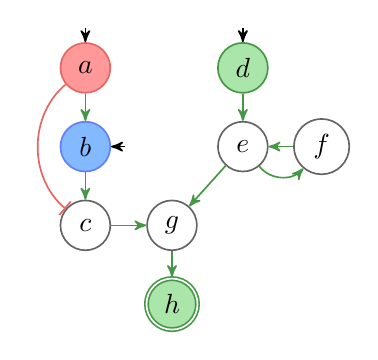
\begin{tikzpicture}[->,semithick,>=stealth',scale=1.0]
    \tikzstyle{label}=[text=black]
    \tikzstyle{species}=[draw=node_gray, circle, minimum size=1.8em, fill=none,text=black]
    \tikzstyle{speciesup}=[style=species,text=black,text opacity=1,fill=node_green,draw=edge_green]
    \tikzstyle{speciesdn}=[style=species,text=black,text opacity=1,fill=node_red,draw=edge_red]
    \tikzstyle{speciesnc}=[style=species,text=black,text opacity=1,fill=node_blue,draw=edge_blue]

    \node[speciesdn] (A) at (0.5,4)  {$a$};
    \node[speciesup] (D) at (2.5,4)  {$d$};
    \node[speciesnc] (B) at (0.5,3)  {$b$};
    \node[species]   (E) at (2.5,3)  {$e$};
    \node[species]   (C) at (0.5,2)  {$c$};
    \node[species]   (F) at (3.5,3)  {$f$};
    \node[species]   (G) at (1.6,2)  {$g$};
    \node[speciesup,accepting] (H) at (1.6,1)  {$h$};

    \path[every node/.style={anchor=south}]
     (0.5,4.5) edge[label=1] (A)
     (1.0,3.0) edge[label=1] (B)
     (2.5,4.5) edge[label=1] (D)
     (A) edge[edge_green] (B)
     (A) edge[edge_red,-|,bend right=50] (C)
     (B) edge[edge_green] (C)
     (D) edge[edge_green] (E)
     (E) edge[edge_green,bend right=50] (F)
     (F) edge[edge_green] (E)
     (C) edge[edge_green] (G)
     (E) edge[edge_green] (G)
     (G) edge[edge_green] (H);

  \end{tikzpicture}

\caption{
Example of an interaction graph with experiment data.
Input variables are marked with a small black arrow.
The color indicates the induced or measured difference between two system states,
 green (increase), red (decrease), blue (0-change).
The readout node is marked with a double circle.
}
\label{fig:complex_example}
\end{center}
\end{figure}


\paragraph*{\bf Inputs and perturbations}

Biological systems react to changes in their environment and to internal
manipulations.
The variables of a system which are controlled externally are called \emph{inputs}
and we denote the set of nodes that represent input variables with $I \subseteq V$.
Because input nodes are controlled externally, they are excluded from the sign
consistency rules.

Perturbations are externally induced changes of the input variables
(e.g.\ by gene knockouts, down regulation, or use of  inhibitors).
The sign of a perturbation signifies the difference to a reference state of the system.
The signs of the perturbation
are defined as $pert: I \rightarrow \{\plus, \minus, 0\}$,
where an increase perturbation $pert(i) = \plus$ (resp. decrease perturbation $pert(i)=\minus$) means that $i$
is controlled such that it has a significant higher (resp. lower) value than in
the reference state.
A special role play so called 0-perturbations with $pert(i)=0$.
These are perturbations where the value of a variable is kept constant.
Such perturbations are particular useful as one can practically ignore the
outgoing edges of 0-perturbed nodes because these nodes can not be responsible
for any downstream changes.
It is easy to see that for complex models with many cyclic interactions such
perturbations are very useful to investigate the influence of single components
while excluding the influence of others.



\paragraph*{\bf Predicting model behaviors}

A prediction function in the sign consistency approach is a function
 $pred: V \times (I \rightarrow \{\plus,\minus,0 \}) \rightarrow 2^{\{\plus,\minus,0 \}}\setminus\emptyset$.
Given a vertex and a perturbation function it returns a nonempty set of possible signs.
The here presented approach is similar to the \emph{dependency matrix}~\cite{sk06}
to make behavioral predictions for initial responses.
We consider pair-wise dependencies among the variables in the IG model.
The relations between two nodes are:
\begin{itemize}
 \item $i$ is an activator of $j$ if there exists a positive elementary path from $i$ to $j$, and
 \item $i$ is an inhibitor of $j$ if there exists a negative elementary path from $i$ to $j$.
\end{itemize}
%
A pair of nodes $i$, $j$ can be in one, both, or none of these relations.
Using these relations our prediction function is defined as follows.
Given a perturbation function $pert: I \rightarrow \{\plus,\minus,0 \}$
 the dependency matrix defines a prediction function
 $pred: V \times (I \rightarrow \{\plus,\minus,0 \}) \rightarrow  2^{\{\plus,\minus,0 \}}\setminus\emptyset $ such that: \\
 $\plus \in pred(j,pert)$ if
\begin{itemize}
  \item $pert(j)=\plus$, or
  \item $j \notin I$ and $\exists i \in I$ and $pert(i)=\plus$  and $i$ is an activator of $j$, or
  \item $j \notin I$ and $\exists i \in I$ and $pert(i)=\minus$ and $i$ is an inhibitor of $j$.
\end{itemize}
  $\minus \in pred(j,pert)$ if
\begin{itemize}
  \item $pert(j)=\minus$, or
  \item $j \notin I$ and $\exists i \in I$ and $pert(i)=\minus$ and $i$ is an activator of $j$, or
  \item $j \notin I$ and $\exists i \in I$ and $pert(i)=\plus$  and $i$ is an inhibitor of $j$.
\end{itemize}
  $0 \in pred(j,pert)$ if
\begin{itemize}
  \item $pert(j)=0$, or
  \item $j \notin I$ and $\plus \in    pred(j,pert)$ and $\minus \in    pred(j,pert)$, or
  \item $j \notin I$ and $\plus \notin pred(j,pert)$ and $\minus \notin pred(j,pert)$.\\
\end{itemize}
% {
% \setlength\tabcolsep{3.8pt}
% \begin{tabular}{lll}
%  \\
%  $\plus \in pred(j,pert)$  & if & $pert(j)=\plus$, or\\
%                            &    & $j \notin I$ and $\exists i \in I$ and $pert(i)=\plus$  and $i$ is an activator of $j$, or\\
%                            &    & $j \notin I$ and $\exists i \in I$ and $pert(i)=\minus$ and $i$ is an inhibitor of $j$,\\
% \\
%  $\minus \in pred(j,pert)$ & if & $pert(j)=\minus$, or\\
%                            &    & $j \notin I$ and $\exists i \in I$ and $pert(i)=\minus$ and $i$ is an activator of $j$, or\\
%             ~              & ~  & $j \notin I$ and $\exists i \in I$ and $pert(i)=\plus$  and $i$ is an inhibitor of $j$, \\
% \\
%  $0 \in pred(j,pert)$      & if & $pert(j)=0$, or\\
%                            & ~  & $j \notin I$ and $\plus \in    pred(j,pert)$ and $\minus \in    pred(j,pert)$, or \\
%                            &    & $j \notin I$ and $\plus \notin pred(j,pert)$ and $\minus \notin pred(j,pert)$.\\
% \\
% \end{tabular}
% }

In the following we simply write $pred(j)$ instead of $pred(j,pert)$.
This prediction function can predict the behaviors
 increase = $\{\plus\}$,
 decrease = $\{\minus\}$,
 0-change = $\{0\}$, or
 undetermined=$\{\plus,\minus,0 \}$=\am.
In principle sign consistency based methods can also make predictions as
 no-increase          = $\{\minus,0 \}$,
 no-decrease          = $\{\plus,0 \}$, and
 increase-or-decrease = $\{\plus, \minus\}$,
for example when backward propagation is applied~\cite{sthiele15}.
Here we apply only forward propagation (from the inputs to the readouts) and
therefore do not make such predictions.
Figure~\ref{fig:experiment_example} shows three models and their predicted
reaction with respect to perturbations.
It contains examples for each type of prediction.
Model A predicts 0-change in $a$ wrt. Experiment~1: $pred(a)= 0$, because there
exists no activator nor inhibitor of $a$ in $I$.
With respect to Experiment~2,
Model A predicts an increase in $b$: $pred(b)=\plus$, and a decrease in $c$: $pred(c)=\minus$,
because $a$ is an activator of $b$ and an inhibitor of $c$ and $pert(a)=\plus$.
Finally, with respect to Experiment~2, Model A makes no prediction for $d$: $pred(d)=\Asterisk$,
because $a$ can be an activator as well as an inhibitor of $d$.


\paragraph*{\bf Experiment}

An experiment consists of two parts, the experiment setup and the measurements.
The experiment setup describes which perturbations are performed,
 and which species will be measured.
Formally, given an IG model $(V,E,\sigma)$,
 an \emph{experiment setup} is defined as a tuple $(I,pert,R)$ where
 $pert: I \rightarrow \{ \plus, \minus, 0 \}$ describes the performed perturbations,
 and $R\subseteq V$ is the set of readouts  (species which are measured).

The measurements describe the observed difference in the readouts
 between the reference state and the measured state.
Given a set of readout nodes $R \subseteq V$, the measurements define a mapping
 $m : R \rightarrow \{\plus, \minus, 0\}$.
 \footnote{For our approach to discretization and the handling of uncertain observations see~\cite{sthiele15}}
%
Following the sign consistency approach, perturbations and measurements define
constraints on the labeling of the influence graph.
An illustration of an experiment setup is given in Figure~\ref{fig:complex_example}.


\paragraph*{\bf Network inference as optional preprocessing}

The input for \expidesi\ is always a set of candidate models.
One has either given an ad hoc set of candidate models or,
what is mostly (and also in the realistic application described in section 3) the case,
an initial (text book) model and some set of (a priori) measurements from previous experiments.
For the latter case, the given data are often inconsistent with the initial model structure ($m(i) \notin pred(i)$).
Here, based on suitable network inference methods,
these data are then used to generate consistent candidate models which then serve as input for \expidesi.

% While the removal of certain edges can improve the agreement between measurements and
% network topology,
% in some cases, certain inconsistencies can only be resolved if one adds new interactions.
Although \expidesi\ is independent from the model inference method that is used for this purpose,
%  we here generate the initial set of candidate models using OPT\_GRAPH~\cite{samaga13a} a sign-consistency based method for model inference which ensures that all candidate models are consistent with prior experimental data.
 we here generate the initial set of candidate models from prior experimental data using OPT\_GRAPH~\cite{samaga13a} a sign-consistency based method for model inference.
 This allows us to implement the complete workflow of experiment planning using sign consistency methods.
% OPT\_GRAPH~\cite{samaga13a} is a sign consistency based method for network inference,
% that
OPT\_GRAPH
intends to resolve inconsistencies by allowing edge removals and insertions in parallel.
However, as the insertion of new interactions increases the solution space
dramatically in large networks,
OPT\_GRAPH implements a greedy strategy which determines, in each iteration,
the optimal (single) edge whose inclusion in combination with the edge removals,
decreases the fitting error the most.
OPT\_GRAPH then adds this edge permanently and repeats until no further
significant improvement can be obtained by inserting a new edge.
If more than one optimal single edge is found during an iteration, then all alternative solution are tracked and explored by OPT\_GRAPH.


\paragraph*{\bf Discriminative power of an experiment}

If for a given experiment,
two models $M_1$ and $M_2$ have in a readout $i \in R$
different predicted behaviors ($pred_{M_1}(i) \neq pred_{M_2}(i)$),
 we call this a \emph{distinctive readout}.
%Figure~\ref{fig:experiment_example} shows three interaction graph models and
% their predicted behavior for given experiments.
The readout in an experiment is \emph{strongly distinctive} for two models
if both models predict contradictory behaviors ($pred_{M_1}(i) \cap pred_{M_2}(i) = \emptyset$).
For example, in Figure~\ref{fig:experiment_example} in Experiment~1,
readout $e$ is strongly distinctive, Model A  predicts a decrease
while Models B and C predict an increase.
When the experiment is performed the measured behavior of $e$ will
 invalidate at least one of the models.
In Experiment~2 in Figure~\ref{fig:experiment_example}, the readout $c$ is distinctive
but not strongly distinctive, Models A and B predict a decrease while Model C gives an undetermined prediction.
If Experiment~2 is performed the measurements may discard Models A and B if an
increase or 0-change in $c$ is measured, but if a decrease is measured then
all three models are consistent.

While Experiment~1 will in any case invalidate some of the candidate models,
Experiment~2 only has the potential to discriminate some candidates.
We say an experiment is \emph{definitely distinguishing} two models if at
least one \emph{strongly distinctive} readout exists (Experiment 1), and an experiment
 \emph{potentially distinguishing} two networks if at least one
 \emph{distinctive} readout exists but no \emph{strongly distinctive} readout (Experiment 2).
We say an experiment can not distinguish two networks if no distinctive readout exist.

\begin{figure*}[!t]
\begin{center}
\begin{tabular}{cccc}
 ~ & Experiment 1: & Experiment 2: & Experiment 3: \\
 ~ & $pert=\{d\rightarrow \plus \}$ & $pert=\{a\rightarrow\plus\}$ & $pert=\{a\rightarrow\plus, b \rightarrow \minus \}$ \\
 ~ & $R =\{e\}$ & $R =\{c\}$ & $R =\{e\}$ \\
Model A)\\
  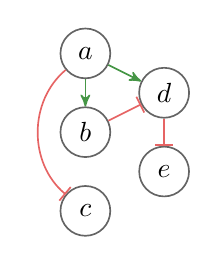
\begin{tikzpicture}[->,semithick,>=stealth',scale=1.0]
    \tikzstyle{label}=[text=black]
    \tikzstyle{species}=[draw=node_gray, circle, minimum size=1.8em, fill=none,text=black]
    \tikzstyle{speciesup}=[style=species,text=black,text opacity=1,fill=node_green,draw=edge_green]
    \tikzstyle{speciesdn}=[style=species,text=black,text opacity=1,fill=node_red,draw=edge_red]
    \tikzstyle{speciesnc}=[style=species,text=black,text opacity=1,fill=node_blue,draw=edge_blue]
    \node[species] (A) at (0.5,4  )  {$a$};
    \node[species] (B) at (0.5,3  )  {$b$};
    \node[species] (C) at (0.5,2  )  {$c$};
    \node[species] (D) at (1.5,3.5)  {$d$};
    \node[species] (E) at (1.5,2.5)  {$e$};

    \path[every node/.style={anchor=south}]
     (A) edge[edge_green] (B)
     (A) edge[edge_red,-|,bend right=50] (C)
     (B) edge[edge_red,-|] (D)
     (A) edge[edge_green] (D)
     (D) edge[edge_red,-|] (E);
  \end{tikzpicture}
&
  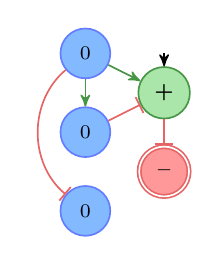
\begin{tikzpicture}[->,semithick,>=stealth',scale=1.0]
    \tikzstyle{label}=[text=black]
    \tikzstyle{species}=[draw, circle, minimum size=1.8em, fill=none,text=black]
    \tikzstyle{speciesup}=[style=species,text=black,text opacity=1,fill=node_green,draw=edge_green]
    \tikzstyle{speciesdn}=[style=species,text=black,text opacity=1,fill=node_red,draw=edge_red]
    \tikzstyle{speciesnc}=[style=species,text=black,text opacity=1,fill=node_blue,draw=edge_blue]
    \tikzstyle{speciesam}=[style=species,text=black,text opacity=1,fill=node_yell,draw=orange]

    \node[speciesnc]           (A) at (0.5,4  )  {\scriptsize $0$};
    \node[speciesnc]           (B) at (0.5,3  )  {\scriptsize $0$};
    \node[speciesnc]           (C) at (0.5,2  )  {\scriptsize $0$};
    \node[speciesup]           (D) at (1.5,3.5)  {\scriptsize $\plus$};
    \node[speciesdn,accepting] (E) at (1.5,2.5)  {\scriptsize $\minus$};

    \path[every node/.style={anchor=south}]
     (A) edge[edge_green] (B)
     (A) edge[edge_red,-|,bend right=50] (C)
     (A) edge[edge_green] (D)
     (B) edge[edge_red,-|] (D)
     (1.5,4.0) edge[label=1] (D)
     (D) edge[edge_red,-|] (E);
  \end{tikzpicture}
&
   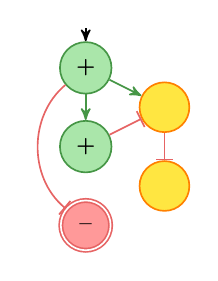
\begin{tikzpicture}[->,semithick,>=stealth',scale=1.0]
    \tikzstyle{label}=[text=black]
    \tikzstyle{species}=[draw, circle, minimum size=1.8em, fill=none,text=black]
    \tikzstyle{speciesup}=[style=species,text=black,text opacity=1,fill=node_green,draw=edge_green]
    \tikzstyle{speciesdn}=[style=species,text=black,text opacity=1,fill=node_red,draw=edge_red]
    \tikzstyle{speciesnc}=[style=species,text=black,text opacity=1,fill=node_blue,draw=edge_blue]
    \tikzstyle{speciesam}=[style=species,text=black,text opacity=1,fill=node_yell,draw=orange]

    \node[speciesup]           (A) at (0.5,4  )  {\scriptsize $\plus$};
    \node[speciesup]           (B) at (0.5,3  )  {\scriptsize $\plus$};
    \node[speciesdn,accepting] (C) at (0.5,2  )  {\scriptsize $\minus$};
    \node[speciesam]           (D) at (1.5,3.5)  {\scriptsize \am};
    \node[speciesam]           (E) at (1.5,2.5)  {\scriptsize \am};

    \path[every node/.style={anchor=south}]
     (0.5,4.5) edge[label=1] (A)
     (A) edge[edge_green] (B)
     (A) edge[edge_red,-|,bend right=50] (C)
     (B) edge[edge_red,-|] (D)
     (A) edge[edge_green] (D)
     (D) edge[edge_red,-|] (E);
  \end{tikzpicture}
&
   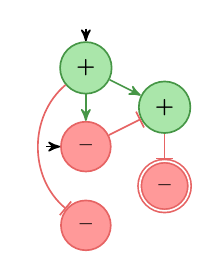
\begin{tikzpicture}[->,semithick,>=stealth',scale=1.0]
    \tikzstyle{label}=[text=black]
    \tikzstyle{species}=[draw, circle, minimum size=1.8em, fill=none,text=black]
    \tikzstyle{speciesup}=[style=species,text=black,text opacity=1,fill=node_green,draw=edge_green]
    \tikzstyle{speciesdn}=[style=species,text=black,text opacity=1,fill=node_red,draw=edge_red]
    \tikzstyle{speciesnc}=[style=species,text=black,text opacity=1,fill=node_blue,draw=edge_blue]
    \tikzstyle{speciesam}=[style=species,text=black,text opacity=1,fill=node_yell,draw=orange]

    \node[speciesup]           (A) at (0.5,4  )  {\scriptsize $\plus$};
    \node[speciesdn]           (B) at (0.5,3  )  {\scriptsize $\minus$};
    \node[speciesdn]           (C) at (0.5,2  )  {\scriptsize $\minus$};
    \node[speciesup]           (D) at (1.5,3.5)  {\scriptsize $\plus$};
    \node[speciesdn,accepting] (E) at (1.5,2.5)  {\scriptsize $\minus$};

    \path[every node/.style={anchor=south}]
     (0.5,4.5) edge[label=1] (A)
     (A) edge[edge_green] (B)
     (A) edge[edge_red,-|,bend right=50] (C)
     (0.0,3.0) edge[label=1] (B)
     (B) edge[edge_red,-|] (D)
     (A) edge[edge_green] (D)
     (D) edge[edge_red,-|] (E);
  \end{tikzpicture}
\\
\\
Model B)\\
  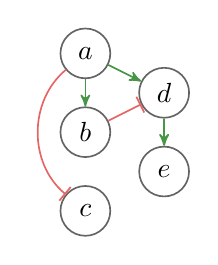
\begin{tikzpicture}[->,semithick,>=stealth',scale=1.0]
    \tikzstyle{label}=[text=black]
    \tikzstyle{species}=[draw=node_gray, circle, minimum size=1.8em, fill=none,text=black]
    \tikzstyle{speciesup}=[style=species,text=black,text opacity=1,fill=node_green,draw=edge_green]
    \tikzstyle{speciesdn}=[style=species,text=black,text opacity=1,fill=node_red,draw=edge_red]
    \tikzstyle{speciesnc}=[style=species,text=black,text opacity=1,fill=node_blue,draw=edge_blue]

    \node[species] (A) at (0.5,4  )  {$a$};
    \node[species] (B) at (0.5,3  )  {$b$};
    \node[species] (C) at (0.5,2  )  {$c$};
    \node[species] (D) at (1.5,3.5)  {$d$};
    \node[species] (E) at (1.5,2.5)  {$e$};

    \path[every node/.style={anchor=south}]
     (A) edge[edge_green] (B)
     (A) edge[edge_red,-|,bend right=50] (C)
     (B) edge[edge_red,-|] (D)
     (A) edge[edge_green] (D)
     (D) edge[edge_green] (E);
  \end{tikzpicture}
&
  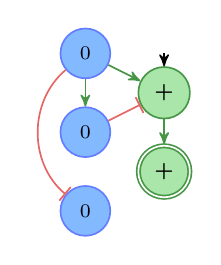
\begin{tikzpicture}[->,semithick,>=stealth',scale=1.0]
    \tikzstyle{label}=[text=black]
    \tikzstyle{species}=[draw, circle, minimum size=1.8em, fill=none,text=black]
    \tikzstyle{speciesup}=[style=species,text=black,text opacity=1,fill=node_green,draw=edge_green]
    \tikzstyle{speciesdn}=[style=species,text=black,text opacity=1,fill=node_red,draw=edge_red]
    \tikzstyle{speciesnc}=[style=species,text=black,text opacity=1,fill=node_blue,draw=edge_blue]
    \tikzstyle{speciesam}=[style=species,text=black,text opacity=1,fill=node_yell,draw=orange]

    \node[speciesnc]           (A) at (0.5,4)    {\scriptsize $0$};
    \node[speciesnc]           (B) at (0.5,3)    {\scriptsize $0$};
    \node[speciesnc]           (C) at (0.5,2)    {\scriptsize $0$};
    \node[speciesup]           (D) at (1.5,3.5)  {\scriptsize $\plus$};
    \node[speciesup,accepting] (E) at (1.5,2.5)  {\scriptsize $\plus$};

    \path[every node/.style={anchor=south}]
     (A) edge[edge_green] (B)
     (A) edge[edge_red,-|,bend right=50] (C)
     (B) edge[edge_red,-|] (D)
     (A) edge[edge_green] (D)
     (1.5,4.0) edge[label=1] (D)
     (D) edge[edge_green] (E);
  \end{tikzpicture}
&
  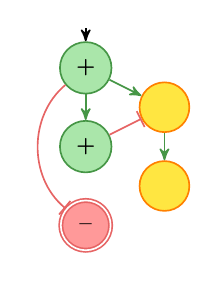
\begin{tikzpicture}[->,semithick,>=stealth',scale=1.0]
    \tikzstyle{label}=[text=black]
    \tikzstyle{species}=[draw, circle, minimum size=1.8em, fill=none,text=black]
    \tikzstyle{speciesup}=[style=species,text=black,text opacity=1,fill=node_green,draw=edge_green]
    \tikzstyle{speciesdn}=[style=species,text=black,text opacity=1,fill=node_red,draw=edge_red]
    \tikzstyle{speciesnc}=[style=species,text=black,text opacity=1,fill=node_blue,draw=edge_blue]
    \tikzstyle{speciesam}=[style=species,text=black,text opacity=1,fill=node_yell,draw=orange]

    \node[speciesup]            (A) at (0.5,4  )  {\scriptsize $\plus$};
    \node[speciesup]            (B) at (0.5,3  )  {\scriptsize $\plus$};
    \node[speciesdn, accepting] (C) at (0.5,2  )  {\scriptsize $\minus$};
    \node[speciesam]            (D) at (1.5,3.5)  {\scriptsize \am};
    \node[speciesam]            (E) at (1.5,2.5)  {\scriptsize \am};

    \path[every node/.style={anchor=south}]
     (0.5,4.5) edge[label=1] (A)
     (A) edge[edge_green] (B)
     (A) edge[edge_red,-|,bend right=50] (C)
     (B) edge[edge_red,-|] (D)
     (A) edge[edge_green] (D)
     (D) edge[edge_green] (E);
  \end{tikzpicture}
&
   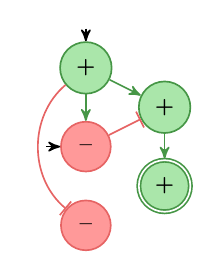
\begin{tikzpicture}[->,semithick,>=stealth',scale=1.0]
    \tikzstyle{label}=[text=black]
    \tikzstyle{species}=[draw, circle, minimum size=1.8em, fill=none,text=black]
    \tikzstyle{speciesup}=[style=species,text=black,text opacity=1,fill=node_green,draw=edge_green]
    \tikzstyle{speciesdn}=[style=species,text=black,text opacity=1,fill=node_red,draw=edge_red]
    \tikzstyle{speciesnc}=[style=species,text=black,text opacity=1,fill=node_blue,draw=edge_blue]
    \tikzstyle{speciesam}=[style=species,text=black,text opacity=1,fill=node_yell,draw=orange]

    \node[speciesup]           (A) at (0.5,4  )  {\scriptsize $\plus$};
    \node[speciesdn]           (B) at (0.5,3  )  {\scriptsize $\minus$};
    \node[speciesdn]           (C) at (0.5,2  )  {\scriptsize $\minus$};
    \node[speciesup]           (D) at (1.5,3.5)  {\scriptsize $\plus$};
    \node[speciesup,accepting] (E) at (1.5,2.5)  {\scriptsize $\plus$};

    \path[every node/.style={anchor=south}]
     (0.0,3.0) edge[label=1] (B)
     (0.5,4.5) edge[label=1] (A)
     (A) edge[edge_green] (B)
     (A) edge[edge_red,-|,bend right=50] (C)
     (B) edge[edge_red,-|] (D)
     (A) edge[edge_green] (D)
     (D) edge[edge_green] (E);
  \end{tikzpicture}
\\
\\
Model C)\\
  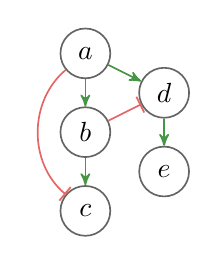
\begin{tikzpicture}[->,semithick,>=stealth',scale=1.0]
    \tikzstyle{label}=[text=black]
    \tikzstyle{species}=[draw=node_gray, circle, minimum size=1.8em, fill=none,text=black]
    \tikzstyle{speciesup}=[style=species,text=black,text opacity=1,fill=node_green,draw=edge_green]
    \tikzstyle{speciesdn}=[style=species,text=black,text opacity=1,fill=node_red,draw=edge_red]
    \tikzstyle{speciesnc}=[style=species,text=black,text opacity=1,fill=node_blue,draw=edge_blue]

    \node[species] (A) at (0.5,4)  {$a$};
    \node[species] (B) at (0.5,3)  {$b$};
    \node[species] (C) at (0.5,2)  {$c$};
    \node[species] (D) at (1.5,3.5)  {$d$};
    \node[species] (E) at (1.5,2.5)  {$e$};

    \path[every node/.style={anchor=south}]
%      (1.0,4.5) edge[label=1] (A)
     (A) edge[edge_green] (B)
     (A) edge[edge_red,-|,bend right=50] (C)
     (B) edge[edge_green] (C)
     (B) edge[edge_red,-|] (D)
     (A) edge[edge_green] (D)
     (D) edge[edge_green] (E);
  \end{tikzpicture}
&
  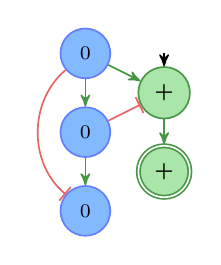
\begin{tikzpicture}[->,semithick,>=stealth',scale=1.0]
    \tikzstyle{label}=[text=black]
    \tikzstyle{species}=[draw, circle, minimum size=1.8em, fill=none,text=black]
    \tikzstyle{speciesup}=[style=species,text=black,text opacity=1,fill=node_green,draw=edge_green]
    \tikzstyle{speciesdn}=[style=species,text=black,text opacity=1,fill=node_red,draw=edge_red]
    \tikzstyle{speciesnc}=[style=species,text=black,text opacity=1,fill=node_blue,draw=edge_blue]
    \tikzstyle{speciesam}=[style=species,text=black,text opacity=1,fill=node_yell,draw=orange]

    \node[speciesnc]            (A) at (0.5,4  )  {\scriptsize $0$};
    \node[speciesnc]            (B) at (0.5,3  )  {\scriptsize $0$};
    \node[speciesnc]            (C) at (0.5,2  )  {\scriptsize $0$};
    \node[speciesup]            (D) at (1.5,3.5)  {\scriptsize $\plus$};
    \node[speciesup, accepting] (E) at (1.5,2.5)  {\scriptsize $\plus$};

    \path[every node/.style={anchor=south}]
     (A) edge[edge_green] (B)
     (A) edge[edge_red,-|,bend right=50] (C)
     (B) edge[edge_green] (C)
     (B) edge[edge_red,-|] (D)
     (A) edge[edge_green] (D)
     (1.5,4.0) edge[label=1] (D)
     (D) edge[edge_green] (E);
  \end{tikzpicture}
&
  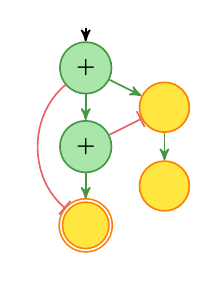
\begin{tikzpicture}[->,semithick,>=stealth',scale=1.0]
    \tikzstyle{label}=[text=black]
    \tikzstyle{species}=[draw, circle, minimum size=1.8em, fill=none,text=black]
    \tikzstyle{speciesup}=[style=species,text=black,text opacity=1,fill=node_green,draw=edge_green]
    \tikzstyle{speciesdn}=[style=species,text=black,text opacity=1,fill=node_red,draw=edge_red]
    \tikzstyle{speciesnc}=[style=species,text=black,text opacity=1,fill=node_blue,draw=edge_blue]
    \tikzstyle{speciesam}=[style=species,text=black,text opacity=1,fill=node_yell,draw=orange]

    \node[speciesup]            (A) at (0.5,4  )  {\scriptsize $\plus$};
    \node[speciesup]            (B) at (0.5,3  )  {\scriptsize $\plus$};
    \node[speciesam, accepting] (C) at (0.5,2  )  {\scriptsize \am};
    \node[speciesam]            (D) at (1.5,3.5)  {\scriptsize \am};
    \node[speciesam]            (E) at (1.5,2.5)  {\scriptsize \am};

    \path[every node/.style={anchor=south}]
     (0.5,4.5) edge[label=1] (A)
     (A) edge[edge_green] (B)
     (A) edge[edge_red,-|,bend right=50] (C)
     (B) edge[edge_green] (C)
     (B) edge[edge_red,-|] (D)
     (A) edge[edge_green] (D)
     (D) edge[edge_green] (E);
  \end{tikzpicture}
&
   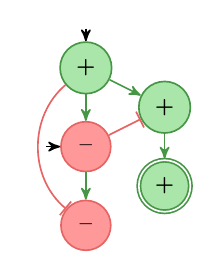
\begin{tikzpicture}[->,semithick,>=stealth',scale=1.0]
    \tikzstyle{label}=[text=black]
    \tikzstyle{species}=[draw, circle, minimum size=1.8em, fill=none,text=black]
    \tikzstyle{speciesup}=[style=species,text=black,text opacity=1,fill=node_green,draw=edge_green]
    \tikzstyle{speciesdn}=[style=species,text=black,text opacity=1,fill=node_red,draw=edge_red]
    \tikzstyle{speciesnc}=[style=species,text=black,text opacity=1,fill=node_blue,draw=edge_blue]
    \tikzstyle{speciesam}=[style=species,text=black,text opacity=1,fill=node_yell,draw=orange]

    \node[speciesup]           (A) at (0.5,4  )  {\scriptsize $\plus$};
    \node[speciesdn]           (B) at (0.5,3  )  {\scriptsize $\minus$};
    \node[speciesdn]           (C) at (0.5,2  )  {\scriptsize $\minus$};
    \node[speciesup]           (D) at (1.5,3.5)  {\scriptsize $\plus$};
    \node[speciesup,accepting] (E) at (1.5,2.5)  {\scriptsize $\plus$};

    \path[every node/.style={anchor=south}]
     (0.0,3.0) edge[label=1] (B)
     (0.5,4.5) edge[label=1] (A)
     (A) edge[edge_green] (B)
     (A) edge[edge_red,-|,bend right=50] (C)
     (B) edge[edge_green] (C)
     (B) edge[edge_red,-|] (D)
     (A) edge[edge_green] (D)
     (D) edge[edge_green] (E);
  \end{tikzpicture}
\\
\end{tabular}

\caption{
Three interaction graph models which can be distinguished experimentally.
Predicted behaviors and experimental conditions are represented as colors on
 the nodes, green (increase), red (decrease), blue (0-change), and yellow
 (undetermined).
Perturbations are indicated with a small black arrow and readouts are shown as
 double circles.
For Experiment~1, Model A predicts a decrease in node $e$, while the Models B
 and C predict an increase.
If one measures in Experiment~1 a decrease in $e$ one must discard Model B and C.
Should the experiment result in an increase in $e$ one must discard Model A.
If the Experiment~1 results in a 0-change in $e$ all three models are
 invalidated and new network candidates must be computed.
For Experiment~2 Models A and B predict a decrease in $c$, while Model C makes
 no prediction for $c$.
If Experiment~2 results in an increase or 0-change in $c$ one must discard
 Models A and B.
Should Experiment~2 result in a decrease of $c$ one cannot discriminate any
 of the three models.
%
For Experiment~3 all models predict the same behavior as for Experiment~1, but Experiment~3 uses a different set of perturbations to achieve this readout behavior.
}
\label{fig:experiment_example}
\end{center}
\end{figure*}


We define two functions to approximate the discriminative power
 of an experiment $E$ wrt. a set of candidate models.
% \comment{Verstehe den Satz von Because bis are unknown nicht!
% Experiment führt doch immer zum Readout +, -, oder 0. Garantiert zu einem dieser Ergebnisse. Was soll dann die probability for (...)results? Das es hier um den Informationsgehalt eines Exp geht, ist schon klar. Der erste Halbsatz ist mir aber unklar.
%}
\begin{itemize}
  \item
  $def\_dis(E)$ denotes the number of pairs of candidate models which are
   definitely distinguished by an experiment $E$.
  \item
  $pot\_dis(E)$ denotes the number of pairs of candidate models which can
   potentially be distinguished by $E$.
\end{itemize}
%
Used as optimization criteria, we want to maximize the number of distinguished
candidate models.


\paragraph*{\bf Experiment costs}

Apart from the discriminative power a second optimization criterion is the
costs of the experiments.
This means in the first place minimizing the number of perturbations.
For an experiment $E$, we denote number of perturbations with $cost(E)$.
Revisiting our example in Figure~\ref{fig:experiment_example}, we can see that
the Experiment~3 with $pert=\{a \rightarrow \plus, b \rightarrow \minus \}$ has
the same discriminative power as Experiment~1, but demands more perturbations.
Hence, we might prefer Experiment~1 over Experiment~3.


\paragraph*{\bf The optimal experiment design problem}

The main goal of optimal experiment design is to find the experiments that are
most likely to discard the most models.
We want to maximize the number of \emph{definitely distinguishable} models and
with a lower priority maximize the number of \emph{potentially distinguishable}
models, and as a third objective we want to minimize the costs.

Formally, given
 a set $\cand$ of candidate models,
 a set $\done$ of already performed experiments,
 a function $ppert: V \rightarrow 2^{\{\plus,\minus,0\}}$ indicating the possible perturbations for a species, and
 a set $\pr$ of possible readouts.
We want to find experiments $E=(I,pert,R) \notin \done$, with
 $pert(i) \in ppert(i)$ for all $i \in I$, and
 $R \subseteq \pr$
 that
 \begin{itemize}
  \item[1.] maximize $def\_dis(E)$,
  \item[2.] maximize $pot\_dis(E)$, and
  \item[3.] minimize $cost(E)$.
 \end{itemize}
%
The optimization problem can be performed using solvers that natively support
hierarchical optimization.
Alternatively, hierarchical optimization could be emulated  with a single linear
optimization function using factors $\alpha, \beta, \gamma$:
\begin{itemize}
  \item[] maximize $\alpha \cdot def\_dis(E)+ \beta \cdot pot\_dis(E) + \gamma \cdot cost(E)$.
\end{itemize}
If the single objective function is used, the factors $\alpha, \beta, \gamma$ can always be chosen such
that the hierarchical ordering among the solutions is ensured.

Note that the problem definition for optimal single experiments can be straightforwardly
extended to optimal sets of experiments.
Then we are looking for a set of experiments which maximizes the discriminative
power while minimizing the number of experiments and perturbations.

While for \emph{definite distinctions} one strongly distinctive readout is
sufficient to distinguish two models,
for \emph{potential distinctions} more distinctive readouts can increase the
probability of an experimental result that allows to distinguish two models.
Therefore, another goal might be to maximize the overall number of
\emph{distinctive} readouts.
%\comment{Not implemented!}


\paragraph*{\bf Relevant perturbations}

Because the measurements of a potentially distinguishing readout might not lead to the invalidation of a model,
experiments containing irrelevant perturbations might be proposed in a subsequent planning step.
For example, in Figure~\ref{fig:redundancy}, Experiment~1 aims to distinguish the Models A and B,
using the measurement of readout $c$,
but a measurement $m(c)=\plus$ does invalidate none of the models.
Therefore, a subsequent planning step might propose Experiment~2.
Although Experiment~2 leads to different predictions as Experiment~1,
we want to discard Experiment~2 because the perturbation in $d$ does not effect any distinctive readout.
Therefore, we use an additional constraint to exclude perturbations that have
in no candidate model a path to a distinctive readout.
%
\begin{figure}[]
\begin{center}
\begin{tabular}{ccc}
 ~ & Experiment 1: & Experiment 2: \\
 ~ & $pert=\{a\rightarrow \plus \}$ & $pert=\{a\rightarrow\plus, d \rightarrow \minus \}$ \\
 ~ & $R =\{c\}$ & $R =\{c\}$ \\
Model A)
\\
  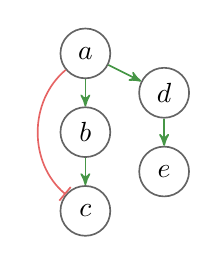
\begin{tikzpicture}[->,semithick,>=stealth',scale=1.0]
    \tikzstyle{label}=[text=black]
    \tikzstyle{species}=[draw=node_gray, circle, minimum size=1.8em, fill=none,text=black]
    \tikzstyle{speciesup}=[style=species,text=black,text opacity=1,fill=node_green,draw=edge_green]
    \tikzstyle{speciesdn}=[style=species,text=black,text opacity=1,fill=node_red,draw=edge_red]
    \tikzstyle{speciesnc}=[style=species,text=black,text opacity=1,fill=node_blue,draw=edge_blue]

    \node[species] (A) at (0.5,4  )  {$a$};
    \node[species] (B) at (0.5,3  )  {$b$};
    \node[species] (C) at (0.5,2  )  {$c$};
    \node[species] (D) at (1.5,3.5)  {$d$};
    \node[species] (E) at (1.5,2.5)  {$e$};

    \path[every node/.style={anchor=south}]
     (A) edge[edge_green] (B)
     (B) edge[edge_green] (C)
     (A) edge[edge_red,-|,bend right=50] (C)
     (A) edge[edge_green] (D)
     (D) edge[edge_green] (E);
  \end{tikzpicture}
&
   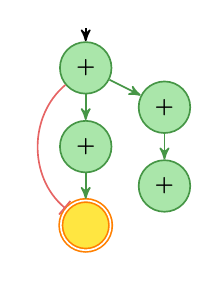
\begin{tikzpicture}[->,semithick,>=stealth',scale=1.0]
    \tikzstyle{label}=[text=black]
    \tikzstyle{species}=[draw, circle, minimum size=1.8em, fill=none,text=black]
    \tikzstyle{speciesup}=[style=species,text=black,text opacity=1,fill=node_green,draw=edge_green]
    \tikzstyle{speciesdn}=[style=species,text=black,text opacity=1,fill=node_red,draw=edge_red]
    \tikzstyle{speciesnc}=[style=species,text=black,text opacity=1,fill=node_blue,draw=edge_blue]
    \tikzstyle{speciesam}=[style=species,text=black,text opacity=1,fill=node_yell,draw=orange]

    \node[speciesup]           (A) at (0.5,4  )  {\scriptsize $\plus$};
    \node[speciesup]           (B) at (0.5,3  )  {\scriptsize $\plus$};
    \node[speciesam,accepting] (C) at (0.5,2  )  {\scriptsize \am};
    \node[speciesup]           (D) at (1.5,3.5)  {\scriptsize $\plus$};
    \node[speciesup]           (E) at (1.5,2.5)  {\scriptsize $\plus$};

    \path[every node/.style={anchor=south}]
     (0.5,4.5) edge[label=1] (A)
     (A) edge[edge_green] (B)
     (B) edge[edge_green] (C)
     (A) edge[edge_red,-|,bend right=50] (C)
     (A) edge[edge_green] (D)
     (D) edge[edge_green] (E);
  \end{tikzpicture}
&
   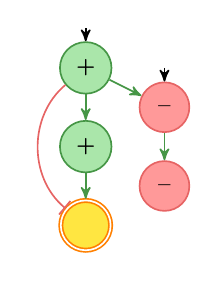
\begin{tikzpicture}[->,semithick,>=stealth',scale=1.0]
    \tikzstyle{label}=[text=black]
    \tikzstyle{species}=[draw, circle, minimum size=1.8em, fill=none,text=black]
    \tikzstyle{speciesup}=[style=species,text=black,text opacity=1,fill=node_green,draw=edge_green]
    \tikzstyle{speciesdn}=[style=species,text=black,text opacity=1,fill=node_red,draw=edge_red]
    \tikzstyle{speciesnc}=[style=species,text=black,text opacity=1,fill=node_blue,draw=edge_blue]
    \tikzstyle{speciesam}=[style=species,text=black,text opacity=1,fill=node_yell,draw=orange]

    \node[speciesup]           (A) at (0.5,4  )  {\scriptsize $\plus$};
    \node[speciesup]           (B) at (0.5,3  )  {\scriptsize $\plus$};
    \node[speciesam,accepting] (C) at (0.5,2  )  {\scriptsize \am};
    \node[speciesdn]           (D) at (1.5,3.5)  {\scriptsize $\minus$};
    \node[speciesdn]           (E) at (1.5,2.5)  {\scriptsize $\minus$};

    \path[every node/.style={anchor=south}]
     (0.5,4.5) edge[label=1] (A)
     (A) edge[edge_green] (B)
     (B) edge[edge_green] (C)
     (A) edge[edge_red,-|,bend right=50] (C)
     (A) edge[edge_green] (D)
     (1.5,4.0) edge[label=1] (D)
     (D) edge[edge_green] (E);
  \end{tikzpicture}
\\
\\
Model B)
\\
  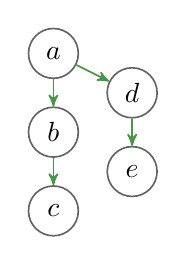
\begin{tikzpicture}[->,semithick,>=stealth',scale=1.0]
    \tikzstyle{label}=[text=black]
    \tikzstyle{species}=[draw=node_gray, circle, minimum size=1.8 em, fill=none,text=black]
    \tikzstyle{speciesup}=[style=species,text=black,text opacity=1,fill=node_green,draw=edge_green]
    \tikzstyle{speciesdn}=[style=species,text=black,text opacity=1,fill=node_red,draw=edge_red]
    \tikzstyle{speciesnc}=[style=species,text=black,text opacity=1,fill=node_blue,draw=edge_blue]

    \node[species] (A) at (0.5,4  )  {$a$};
    \node[species] (B) at (0.5,3  )  {$b$};
    \node[species] (C) at (0.5,2  )  {$c$};
    \node[species] (D) at (1.5,3.5)  {$d$};
    \node[species] (E) at (1.5,2.5)  {$e$};

    \path[every node/.style={anchor=south}]
     (A) edge[edge_green] (B)
     (B) edge[edge_green] (C)
     (A) edge[edge_green] (D)
     (D) edge[edge_green] (E);
  \end{tikzpicture}
&
  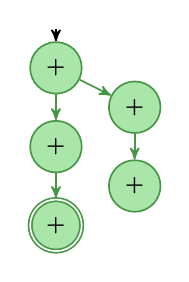
\begin{tikzpicture}[->,semithick,>=stealth',scale=1.0]
    \tikzstyle{label}=[text=black]
    \tikzstyle{species}=[draw, circle, minimum size=1.8 em, fill=none,text=black]
    \tikzstyle{speciesup}=[style=species,text=black,text opacity=1,fill=node_green,draw=edge_green]
    \tikzstyle{speciesdn}=[style=species,text=black,text opacity=1,fill=node_red,draw=edge_red]
    \tikzstyle{speciesnc}=[style=species,text=black,text opacity=1,fill=node_blue,draw=edge_blue]
    \tikzstyle{speciesam}=[style=species,text=black,text opacity=1,fill=node_yell,draw=orange]

    \node[speciesup]           (A) at (0.5,4  )  {\scriptsize $\plus$};
    \node[speciesup]           (B) at (0.5,3  )  {\scriptsize $\plus$};
    \node[speciesup,accepting] (C) at (0.5,2  )  {\scriptsize $\plus$};
    \node[speciesup]           (D) at (1.5,3.5)  {\scriptsize $\plus$};
    \node[speciesup]           (E) at (1.5,2.5)  {\scriptsize $\plus$};

    \path[every node/.style={anchor=south}]
     (0.5,4.5) edge[label=1] (A)
     (A) edge[edge_green] (B)
     (B) edge[edge_green] (C)
     (A) edge[edge_green] (D)
     (D) edge[edge_green] (E);
  \end{tikzpicture}
&
  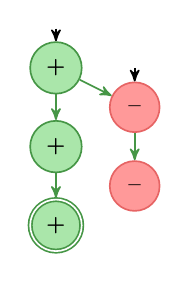
\begin{tikzpicture}[->,semithick,>=stealth',scale=1.0]
    \tikzstyle{label}=[text=black]
    \tikzstyle{species}=[draw, circle, minimum size=1.8 em, fill=none,text=black]
    \tikzstyle{speciesup}=[style=species,text=black,text opacity=1,fill=node_green,draw=edge_green]
    \tikzstyle{speciesdn}=[style=species,text=black,text opacity=1,fill=node_red,draw=edge_red]
    \tikzstyle{speciesnc}=[style=species,text=black,text opacity=1,fill=node_blue,draw=edge_blue]
    \tikzstyle{speciesam}=[style=species,text=black,text opacity=1,fill=node_yell,draw=orange]

    \node[speciesup]           (A) at (0.5,4  )  {\scriptsize $\plus$};
    \node[speciesup]           (B) at (0.5,3  )  {\scriptsize $\plus$};
    \node[speciesup,accepting] (C) at (0.5,2  )  {\scriptsize $\plus$};
    \node[speciesdn]           (D) at (1.5,3.5)  {\scriptsize $\minus$};
    \node[speciesdn]           (E) at (1.5,2.5)  {\scriptsize $\minus$};

    \path[every node/.style={anchor=south}]
     (0.5,4.5) edge[label=1] (A)
     (A) edge[edge_green] (B)
     (B) edge[edge_green] (C)
     (A) edge[edge_green] (D)
     (1.5,4.0) edge[label=1] (D)
     (D) edge[edge_green] (E);
  \end{tikzpicture}
\\
\end{tabular}

 \caption{
 Two interaction graph models which are potentially distinguished by Experiments~1 and 2.
 The predicted behaviors and experimental conditions are represented as colors on the nodes,
 green (increase), red (decrease), blue (0-change), and yellow (undetermined).
 Perturbations are indicated with a black incoming edge.
 For Experiments~1 and 2 Model A predicts an undetermined behavior in node $c$
  while Model B predicts an increase in $c$.
 Both experiments may distinguish Model A and B but for the minimal number of perturbations one would prefer
 Experiment~1.
 Experiment~2 is redundant, even if Experiment~1 fails to distinguish the two models (because $c$ is measured \plus)
 Experiment~2 is not capable to cause a different behavior in any readout.
 The only difference between Experiment~1 and 2 is a perturbation in $d$ which has in none of the models a path to a distinctive readout.
 }
\label{fig:redundancy}
\end{center}
\end{figure}



\paragraph*{\bf Implementation}

To solve the optimal experiment design problem we formulated it
by means of Answer Set Programming (ASP)~\cite{baral02a}.
ASP is a declarative problem solving paradigm from the field of logic
programming and knowledge representation, that offers a rich modeling
language~\cite{potasscoManual} along with highly efficient inference
engines~\cite{gekanesc07a} based on Boolean constraint solving technology.
We provide a python program called \expidesi~that uses the ASP solver through
the PyASP library.
\expidesi~is open source and available as part of the BioASP software collection at
\texttt{https://github.com/bioasp/exdesi}.




\section{Case study: Erythropoietin signal transduction}

We tested our approach to optimal experiment design using the model of the
Erythropoietin signal transduction in the cell line \texttt{HEK293} derived from
human embryonic kidney cells.
Erythropoietin (Epo) is a cytokine which initiates red blood cell generation and
thus adjusts the capacity of the blood to transport oxygen.
The Epo-encoding gene is activated in case of hypoxia in the kidney and liver by
the transcription factor HIF (hypoxia induced factor).
Epo acts on erythroid progenitor cells which finally develop to reticulocytes\cite{wib1}.
This differentiation depends on binding of Epo to the transmembrane Epo receptor.
The receptor does not harbour intrinsic kinase activity but is constitutively
associated with the tyrosine kinase JAK2 (Janus kinase 2).
After binding of Epo to the receptor, JAK2 is tyrosine phosphorylated and thus activated.
JAK2 subsequently phosphorylates and activates the transcription factors signal
transducer and activator of transcription (STAT)3 and 5.
A negative feedback is implemented by the induction of the STAT-dependent feedback
inhibitors SOCS3 and CIS\cite{wib2}.
The regulation of the STAT-independent signalling modules involves the multi-site
docking proteins of the Gab (Grb2 associated binder) family\cite{wib3}.
Gab-proteins contribute to the coordination and activation of the PI3K/AKT pathway,
the MAPK-cascade, and the PLC-cascade.
The detailed interconnection of these signalling modules is not fully understood, yet.
In brief, Gab proteins are recruited to the plasma membrane and there act as a
signalling platform by binding Grb2/SOS, SHP2, PI3K, PLC and other signalling
components.
Several regulatory loops are predicted as e.g. Gab binding to PIP3 in the plasma
membrane depends on PI3K- and MAPK-activity\cite{wib4}.
The original model that served as our gold standard was given in form of a
Boolean network (BN).
The hypergraph representation of the Boolean network contains $23$ species and
$28$ hyperarcs.
In Boolean networks the underlying interaction graphs can easily be obtained\cite{sk06}.

A realistic experimental setup involves the following list of possible
perturbations and readouts.
\begin{itemize}
  \item
  nine possible down-regulations (e.g.\ by use of suitable inhibitors):
  {\sffamily akt},
  {\sffamily mek1},
  {\sffamily mtorc1},
  {\sffamily pi3k},
  {\sffamily gab1\_ps},
  {\sffamily gab1\_bras\_py},
  {\sffamily gab1\_bpi3k\_py},
  {\sffamily shp2, shp2\_ph},
  \item
  three possible up-regulations:
  {\sffamily gab1\_ps},
  {\sffamily shp2},
  {\sffamily shp2\_ph}, and
  \item eight possible readouts:
  {\sffamily akt},
  {\sffamily erk},
  {\sffamily gab1\_bshp2\_ph\_py},
  {\sffamily gab1\_ps},
  {\sffamily jak2\_p},
  {\sffamily plcg},
  {\sffamily shp2},
  {\sffamily stat5ab\_py}.\end{itemize}

In the first part of this case study,
we used \emph{in silico} experiments to validate our approach by creating a
distorted version of the gold standard and then planning experiments that
restored the gold standard.
In the second part, we planned \emph{in vivo} experiments to refine our
knowledge of the Erythropoietin signaling pathway in \texttt{HEK293} cells.


\subsection{\emph{In silico} experiments}

We tested our approach \emph{in silico} by restoring the gold standard model
of the Erythropoietin signal transduction from a distorted version of the model.
We performed quantitative simulations of the proposed experiments using an
ODE system which was created from the gold standard.
A detailed description of the \emph{in silico} study is given in the following:

\begin{itemize}
  \item First, we created an ODE system from the gold standard BN using the software ODEfy\cite{odefy}.
  \item This ODE model of the gold standard was used to simulate three initial experiments and subsequently
the experiments that were proposed by our experiment design procedure.

We identified a steady state in the ODE system,
which we used as initial state of the system in our simulated experiments.
In order to simulate the perturbation at time point 0,
we fixed the variables for the perturbed species to constants such that
increased species had a value significantly higher than in the initial state,
decreased species a value %$0.1$ times the value
significantly lower than in initial state, and
0-perturbed species were kept constant as in the initial state.
We restarted the simulation using these perturbed values and tracked the sign
of the first change of the dependent system variables as initial response.
%\comment{Sven: Add after how much time, how many timesteps? parameters of steady-state!}

The three initial experiments were
1) an increase of {\sffamily mek1},
2) a decrease of {\sffamily pi3k}, and
3) the simultaneous decrease of {\sffamily mek1} and {\sffamily pi3k}.

  \item As starting point for experiment planning and model reconstruction,
we transformed the gold standard BN into an influence graph which consists of
 $23$ nodes and $51$ edges (Figure~\ref{fig:goldVSdistorted}a).
%The compressed IG model consisted of
% $23$ nodes and $51$ edges.
We then created a distorted version (Figure~\ref{fig:goldVSdistorted}b) where
we removed the edge ({\sffamily erk} $\rightarrow$ {\sffamily gab1\_ps}) and added two new edges
 ({\sffamily mek1} $\dashv$ {\sffamily shp2}) and
 ({\sffamily mek1} $\rightarrow$ {\sffamily stat5ab\_py}).
%\comment{Wiebke:Ist es notwendig zu erläutern was gab1\_ps oder stat5ab-py und später folgende bedeuten?}
%\comment[Sven: nur auf nachfrage!}
These wrong/missing edges needed to be identified by the inference method.
%The influence graph of the gold standard model and the distorted version are
%shown side by side in Figure~\ref{fig:goldVSdistorted}.



%  \item We used the ODE model of the gold standard to simulate three
%realistic experiments.
%As expected the results of the simulated experiment were consistent with our
%IG model of the gold standard but inconsistent with the distorted IG model.

  \item We used the OPT\_GRAPH method for network inference on the distorted model
together with the data of the initial experiments.
As expected the data of the simulated experiment were consistent with our
gold standard but inconsistent with the distorted IG model.
OPT\_GRAPH proposed six candidate models that were consistent with the initial experiment data.
Note, that in our case the gold standard IG was among those candidate models,
which is not guaranteed by the OPT\_GRAPH method.

  \item We started the first round of experiment planning,
with these six candidate models including the constraints on possible perturbations and
readouts.
In the first round an experimental setup with one perturbation (decrease of {\sffamily akt} via {\sffamily akt\_inhibitor}) was proposed.
Figure~\ref{tab:predictions_allexp} shows the predicted behaviors
for the six network candidates in the proposed experiment.
The simulation results of the proposed experiment were consistent with three
models (4, 5, 6) and could exclude three candidates (1, 2, 3).

  \item In the second round of experiment planning two experiments with two perturbations
distinguishing two classes of models were proposed.
Figure~\ref{tab:predictions_allexp} shows the predicted behaviors for one of
the proposed experiments (simultaneous decrease of {\sffamily gab1\_bras\_py} and {\sffamily shp2}).
The simulation results of the proposed experiment were consistent with two
models (4, 5) and could exclude one candidate (6).

This point marks the limit of what is currently technically possible.
We have had exhausted all the perturbation and measuring methods available to
the wet lab.
It would not be possible to distinguish the remaining models.
However our ODE model does not succumb to these restrictions as we can observe
and perturb all components.

  \item We continued the third round of experiment planning dropping all restrictions
on possible perturbations.
Two experiment setups distinguishing the maximal number of two classes of models
with the minimum of two perturbations were proposed.
The Figure~\ref{tab:predictions_allexp} shows the predicted behaviors for one of
the proposed experiments (simultaneous increase of {\sffamily erk} and decrease of {\sffamily mek}).
Finally, the predictions of only one model is consistent with the results of
the simulated experiment,
model $5$ which is identical to our gold standard.

\end{itemize}

\begin{figure}[h]
\begin{center}
 \includegraphics[scale=.45,keepaspectratio=true]{./figures/gold_standard_IG.pdf}
 ~~~
 \includegraphics[scale=.45,keepaspectratio=true]{./figures/distorted_IG.pdf}

 \caption{
   The influence graph model of the gold standard (a) and the distorted version (b).
   Added edges are drawn thicker and removed edges are striked out.
 }
 \label{fig:goldVSdistorted}
\end{center}
\end{figure}

\begin{figure}[h]
\begin{center}
\sffamily
\small
\begin{tabular}{c|c|c| c|c|c| c|c|c|}
~ & \multicolumn{2}{c|}{Experiment 1} & \multicolumn{3}{c|}{Experiment 2} & \multicolumn{3}{c|}{Experiment 3} \\
~ & pert. & read & \multicolumn{2}{c|}{pert.} & read & \multicolumn{2}{c|}{pert.} & read \\
  model id & \rot{akt\_inhibitor} &  \rot{gab1\_ps}
           & \rot{gab1\_bras\_py} & \rot{shp2} &\rot{gab1\_ps}
           & \rot{erk} & \rot{mek1} & \rot{gab1\_ps} \\
  \hline
5 & $\plus$ & \gc  0       & $\minus$ & $\minus$ & \gc \am & $\plus$ & $\minus$ & \gc $\plus$  \\
4 & $\plus$ & \gc  0       & $\minus$ & $\minus$ & \gc \am & $\plus$ & $\minus$ & \rc $\minus$ \\
% \cline{11-13}
6 & $\plus$ & \gc  0       & $\minus$ & $\minus$ & \rc $\plus$ & \multicolumn{3}{c|}{~} \\
% \cline{8-10}
1 & $\plus$ & \rc $\minus$ & \multicolumn{3}{c|}{~} & \multicolumn{3}{c|}{~} \\
2 & $\plus$ & \rc $\minus$ & \multicolumn{3}{c|}{~} & \multicolumn{3}{c|}{~} \\
3 & $\plus$ & \rc $\minus$ & \multicolumn{3}{c|}{~} & \multicolumn{3}{c|}{~} \\
\hline
  \multicolumn{1}{c}{~} \\
  \multicolumn{2}{c}{~} & \multicolumn{7}{c}{simulation results} \\
  \cline{3-3}\cline{6-6}\cline{9-9}
  \multicolumn{2}{l|}{gold standard} & 0 & \multicolumn{2}{c|}{~} & $\minus$ & \multicolumn{2}{c|}{~} & $\plus$\\
  \cline{3-3}\cline{6-6}\cline{9-9}
\end{tabular}
\end{center}
\caption{
  Results of the \emph{in silico} study. Predicted behavior for the candidate models and behavior of the
  gold standard simulation under the proposed experiment.
  Predictions that are consistent with the simulation results are in green,
  inconsistent predictions are shown red.
}
\label{tab:predictions_allexp}
\end{figure}


\subsection{\emph{In vivo} experiments}

For \emph{in vivo} experimentation,
we started with $26$ model candidates based on the gold standard and existing
experimental data\footnote{online available at:\\ https://github.com/bioasp/iggy/tree/master/data/in\_vivo\_HEK293}.
%\comment{Wiebke: Welche Daten sind das? Ist dafür auch eine genauere Beschreibung notwendig?}
%\comment{Sven: create supplements! Beschreibung nur auf Nachfrage!}
Our experiment planning proposed the experiment shown in Figure~\ref{tab:predictionsWt}
in which the inhibition of {\sffamily akt} would allow us to distinguish two classes
of models and thus to invalidate at least six model candidates.
%
These model classes are illustrated in Figure~\ref{fig:modeltypeAB1}.
All model candidates suggest to introduce a regulation of {\sffamily erk} that was not
present in the gold standard.
The models of class $A$ contain regulations upstream of {\sffamily akt} via
 {\sffamily gab1\_bshp2\_ph\_py},
 {\sffamily gab1\_bpi3k\_py},
 {\sffamily plcg},
 {\sffamily gab1\_bras\_py},
 {\sffamily ras\_gap},
 {\sffamily pi3k} or
 {\sffamily mtor}.
If a model from class $A$ reflects the biological reality,
then an inhibition of {\sffamily akt} should have no effect on {\sffamily erk}.
The models of class $B$ contain a regulation of {\sffamily erk} downstream of
{\sffamily akt}, via
 {\sffamily mtorc1},
 {\sffamily mtorc2} or
 {\sffamily akt} directly.
If a model of class $B$ reflects reality we should see an increase in
{\sffamily erk} and {\sffamily gab1\_ps}.

\begin{figure}[h]
\begin{center}
\sffamily
\small
\begin{tabular}{c|c| c|c|c|c|c|c|}
~ & \multicolumn{1}{c|}{pert.} & \multicolumn{6}{c|}{readout} \\
model id & akt\_inhibitor & \rot{erk} & \rot{jak2\_p} & \rot{plcg} & \rot{gab1\_ps} & \rot{stat5ab\_py} & \rot{shp2} \\
\hline
Class A   &          &         &     &     &         &     &     \\
20 models & $\plus$ &       0 &  0  &  0  & 0       &  0  &  0  \\
          &          &         &     &     &         &     &     \\
Class B   &          &         &     &     &         &     &     \\
6 models  & $\plus$ & $\plus$ & \am & \am & $\plus$ & \am & \am \\

\end{tabular}
\end{center}
\caption{
  Predicted behavior for the candidate models of the Erythropoietin signal
  transduction in \texttt{HEK293} cells in Experiment~1 of the \emph{in vivo} study.
}
\label{tab:predictionsWt}
\end{figure}

\begin{figure}[h]
\begin{center}
 \includegraphics[scale=.45,keepaspectratio=true]{./figures/wt_model_class_A.pdf}

 \includegraphics[scale=.45,keepaspectratio=true]{./figures/wt_model_class_B.pdf}
 \end{center}
 \caption{
   Two model classes for the Erythropoietin signal transduction network in \texttt{HEK293} cells.
   Alternative regulations in different models are shown with black arrows.
   Class $A$ contains regulations of {\sffamily erk} upstream of {\sffamily akt}.
   Class $B$ contains regulations of {\sffamily erk} downstream of {\sffamily akt}.
   Models of class $A$ predict no effect of an inhibition of {\sffamily akt},
   while models of class $B$ predict an increase of {\sffamily erk} and {\sffamily gab1\_ps}.
 }
 \label{fig:modeltypeAB1}
\end{figure}

The experiment was set up and performed according to the computed specification.
\texttt{HEK293} cells expressing JAK2 wild type and the Epo receptor were pre-treated
with the Akt inhibitor MK-2206 (2 $\upmu$M, 30 min) or solvent control before Epo
stimulation (3 U/ml, 15 min).
Cell lysates were prepared and proteins were separated by SDS–PAGE.
After Western blotting, the membranes were stained for phosphorylated forms of
Gab1, JAK2, STAT5, PLC$\upgamma$, SHP2, Erk1/2 and Akt.
Three independent experiments were performed.
The experimental results showed that the inhibition of {\sffamily akt} had no
effect on {\sffamily erk} and {\sffamily gab1\_ps}.
Therefore, we were able to exclude six of the model candidates and perform
a second round of experiment planning trying to discriminate among the remaing
$20$ model candidates.

In the second round our experiment planning proposed the experiment shown in
Figure~\ref{tab:predictionsWt2}.
The proposed inhibition of {\sffamily mtor} distinguished two classes of models.
Promising to invalidate at least two of the model candidates.
The models of class $C$ contain regulations upstream of {\sffamily mtor} via
 {\sffamily gab1\_bshp2\_ph\_py},
 {\sffamily gab1\_bpi3k\_py},
 {\sffamily plcg},
 {\sffamily gab1\_bras\_py},
 {\sffamily ras\_gap} or
 {\sffamily pi3k}.
If a model from class $C$ reflects the biological reality,
then an inhibition of {\sffamily mtor} should have no effect on {\sffamily erk}.
The models of class $D$ contain a regulation of {\sffamily erk} via
{\sffamily mtor}.
If a model of class $D$ reflects reality we should see an increase in
{\sffamily erk} and {\sffamily gab1\_ps}.

\begin{figure}[h]
\begin{center}
\sffamily
\small
\begin{tabular}{c|c| c|c|c|c|c|c|}
~ & \multicolumn{1}{c|}{pert.} & \multicolumn{6}{c|}{readout} \\
model id & {mtor\_inhibitor} & \rot{erk} & \rot{jak2\_p} & \rot{plcg} & \rot{gab1\_ps} & \rot{stat5ab\_py} & \rot{shp2} \\
\hline
Class C   &         &         &     &     &         &     &     \\
18 models & $\plus$ &       0 &  0  &  0  & 0       &  0  &  0  \\
          &         &         &     &     &         &     &     \\
Class D   &         &         &     &     &         &     &     \\
2 models  & $\plus$ & $\plus$ & \am & \am & $\plus$ & \am & \am \\
\end{tabular}
\end{center}
\caption{
  Predicted behavior for the candidate models of the Erythropoietin signal
  transduction in \texttt{HEK293} cells in Experiment~2 of the \emph{in vivo} study.
}
\label{tab:predictionsWt2}
\end{figure}

The experiment was set up and performed according to the computed specification.
\texttt{HEK293} cells expressing JAK2 wild type and the Epo receptor were pre-treated
with the mTOR inhibitor Rapamycin (10 nM, 30 min) or solvent control before Epo
stimulation (3 U/ml, 15 min).
Cell lysates were prepared and proteins were separated by SDS–PAGE.
After Western blotting, the membranes were stained for phosphorylated forms of
Gab1, JAK2, STAT5, PLC$\upgamma$, SHP2, Erk1/2 and Akt.
Three independent experiments were performed.
The experimental results showed that the inhibition of {\sffamily mtor} had
no effect on our readout species.
Therefore, we were able to exclude another two of the model candidates reducing
the candidate set to $18$.

Continued experiment planning proposed further experiments that contained
multiple perturbations which, however, were too complex to conduct with our
facilities.


\subsection{Testing scalability and sensitivity }

To assess the sensitivity and scalability of our approach with respect to different settings
we created 165 distorted models from the gold standard (Figure~\ref{fig:goldVSdistorted}a).
In each distorted model, 1 edge from the gold standard has been deleted and 2 edges not contained
in the gold standard have been added.
For each distorted model we used the OPT\_GRAPH method together with the existing real experimental data
and computed candidate models that correct the inconsistencies with the experimental data.
Figure~\ref{fig:candidates} shows a histogram for the number of candidate models that have been proposed
for the distorted models.

\begin{figure}[h]
\begin{center}
\includegraphics[scale=0.9,keepaspectratio=true]{./figures/histogram.pdf}
\end{center}
\caption{
 Number of candidate models proposed for each of the 165 distorted models.
 For 120 distorted models, OPT\_GRAPH proposed a single candidate model
 while for the remaining 45 distorted models up to 27 repair candidates were identified.
}

\label{fig:candidates}
\end{figure}

42 of the 165 distorted models remained consistent with the data,
and another 78 distorted models were found inconsistent but had only a single optimal repair candidate proposed.
These singleton candidate sets required no experimental design for discrimination.
The remaining 45 distorted models exhibit inconsistencies with the experiments and OPT\_GRAPH proposed
more than one (between 6 and 27) alternative candidate models
that could then be treated with our experimental design approach.

\begin{table*}[!t]

\definecolor{gray}{RGB}{230,230,230}
\begin{center}
\sffamily
\small
\begin{tabular}{cc}
 ~  \\
 \multicolumn{2}{c}{scenario}  \\
 \# readouts & \# pert.\\
 \cellcolor{gray}real (8) & \cellcolor{gray}real (13)\\
 \cellcolor{gray}real (8) & \cellcolor{gray}more (20) \\
 \cellcolor{gray}all (23) & \cellcolor{gray}real (13)\\
 \cellcolor{gray}all (23) & \cellcolor{gray}more (20) \\
 ~  \\
\end{tabular}
~
\begin{tabular}{c}
 a)  \\
 \cellcolor{gray} \% definitely / \% potentially \\
 \cellcolor{gray} distinguishable candidate pairs \\
 12\% / 64\% \\
 14\% / 54\% \\
 53\% / 27\% \\
 64\% / 18\%  \\
 ~  \\
\end{tabular}
~~~~
\begin{tabular}{c}
 b)  \\
 \cellcolor{gray} \# necessary perturbations  \\
 \cellcolor{gray} ~  \\
 2.34  \\
 3.02  \\
 3.36  \\
 5.42  \\
 ~  \\
\end{tabular}
~~~~
\begin{tabular}{c}
 c)  \\
 \cellcolor{gray} \# alternative  experiments  \\
 \cellcolor{gray} ~  \\
 1.8   \\
 1.76  \\
 1     \\
 1.62  \\
 ~  \\
\end{tabular}
\end{center}
\caption{
Results from the randomized benchmark calculations for four different scenarios which are a combination of either 13 realistic perturbations or an extended set of 20 perturbations with either 8 actually used readouts or all 23 nodes as readouts.
All numbers present the average over all 45 candidate sets under the corresponding readout/perturbation scenario.
Column a) shows the percentage of definitely distinguishable pairs of candidates /
the average percentage of (only) potentially distinguishable candidate pairs.
Column b) shows the  number of necessary perturbations (per experiment)
proposed by the optimal experiments.
Column c) shows the average number of alternative optimal experiments found
(per candidate set).}
\label{tab:empirical_study}
\end{table*}

We tested our method with different parameter settings.
Starting with the realistic setup of 8 possible readouts and 13 possible perturbations
we created further scenario combinations,
where all 23 nodes are considered as readouts or/and with increased number (20 instead of 13)
of possible perturbations (the additional perturbations were randomly selected).

For each computed optimal experiment, we recorded how many perturbations
and how many alternative experiments were proposed
and how good the experiment could distinguish among the candidates.
For the latter, we computed for each proposed experiment the portion of pairs of candidate networks
that could be distinguished.
Given the number $n$ of candidates, $all\_pairs = n \times (n-1)/2$ is the number of all possible candidate pairs.
With the number $def\_dis$ of pairs that could be definitely distinguished
with the proposed optimal experiments we computed the ratio $def\_dis / all\_pairs$.
Note that in practice an experiment that can distinguish one network from the rest
can be enough to discriminate $n-1$ candidate pairs.
Such an experiment has thus a discrimination ratio of $2(n-1)/(n \times (n-1)$.
Hence, with increasing $n$ the ratio of such experiments approaches zero.
On the other hand, the more network candidates one has the \emph{easier} it will
be to discriminate at least some of them.

Table~\ref{tab:empirical_study} shows the effect of the different settings
on the ratio of distinguishable candidate pairs, the number of necessary perturbations,
and the number of proposed alternative experiments.

Increasing the number of possible readouts had no significant effect on the runtime
of the optimal experiment computation but, as expected,
resulted in better experiments in the sense that they allow distinguishing more model candidates
(sometimes requiring more perturbations).
Overall, less alternative optimal experiments are proposed when the number of readouts increased.
Hence, the optimal experimental design strategies become more constrained.

Increasing the number of possible perturbation points from 13 to 20 resulted
in experiments by which the model candidates can be better distinguished,
however, the effect was much less pronounced compared to the scenario
where all nodes are considered as readout nodes.
Moreover, in contrast to a higher number of readouts, increasing the number of perturbations has an effect
on the size of the search space of optimal solutions and thus also on the runtime of the computation.
In fact, further increasing the number of possible perturbations in the benchmarks (beyond 20 as used herein)
resulted partially in computation times that exceeded our time limit (1 day).
These results suggest, at least for our case study,
investments in readouts are more rewarding than increasing the number of perturbations.

Importantly, for all 45 sets of candidate models, at least one discriminating experiment could be proposed.
Further conclusions regarding the benchmark study are given in the following Discussion section.







\section{Discussion}

We presented a new approach to experiment planning with multiple perturbations
in the context of interaction graph models.
We demonstrated \emph{in silico} that our planning approach proposes experiments
that are suitable to restore a gold standard model from a distorted model.
Further, we showed \emph{in vivo} that our approach proposes experiments that
allowed us to systematically reduce our space of possible models for the
Erythropoietin signal transduction in \texttt{HEK293} cells and
to exclude certain interactions.

In an empirical study, we showed that while the approach is sensitive to the number of possible perturbations,
it works robustly on problems of realistic sizes.
For all the tested candidate sets at least one discriminating experiment could be proposed.
\texttt{ExDesi} is easily scalable in the number of possible readouts which, as expected,
also leads to much better results.
In contrast, the approach has only limited scalability in the number of possible perturbations
since increasing those leads to an exponential growth of the search space.
We are confident that future research and the progress in the used solver technology
will allow us to scale this approach to problems with larger search spaces.

Generally, as holds true for many model discrimination methods,
models which are underconstrained (e.g., because there are too many candidate edges in the initial graph)
can usually not be falsified because the model explains all observed behaviors.
Thus, it is very important to start with a sparse model
where (most) included interactions have a relatively high confidence.

Only few methods for the selection of optimal sets of multiple perturbations have
been proposed so far.
\texttt{MEED}~\cite{szczurek2009} is an approach that uses ternary logic networks and microarray data.
\texttt{Caspo}~\cite{videla2015} on the other hand uses Boolean logic networks and Boolean data (on and off) within a single state of the biological system.
In contrast, our method is based on interaction graphs and uses data on (signed) changes (ups and downs between two states) as response to perturbations.
\texttt{ExDesi} is to a certain degree related to \texttt{Caspo} as both work on topological similar models (Boolean networks transformed to interaction graphs),
but one cannot easily extract a Boolean state from data expressing signed changes.
For example the sign for an increased value in a variable can be interpreted as a Boolean variable that switches from an OFF state to an ON state,
but depending on the thresholds used to mark the border between ON and OFF it could also refer to a variable that remains in its initial OFF/ON state.

\begin{figure}[]
\begin{center}
  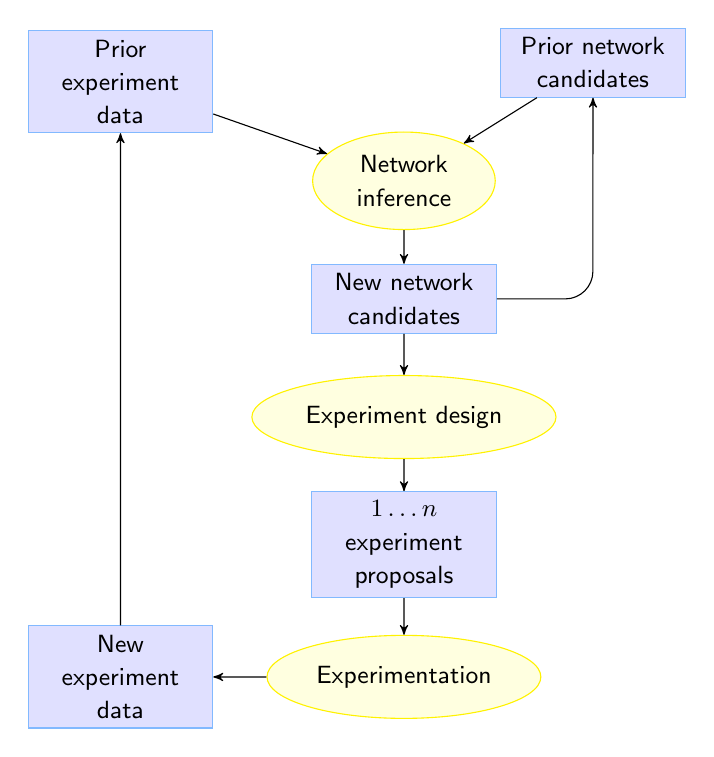
\begin{tikzpicture}[->,>=stealth',scale=1.2]
    \sffamily
    \tikzstyle{label}=[text=black]
    \tikzstyle{wht}=[draw=none, fill=none,text=black,text opacity=1,text=black]
    \tikzstyle{bbox}=[draw=yellow,ellipse,minimum height=3em, text opacity=1,fill=lightyellow,text=black, text badly centered]
    \tikzstyle{box}=[draw=node_blue,rectangle,minimum height=2em,text opacity=1,fill=lightblue,text=black, text badly centered, text width=6em]
    \tikzstyle{decision}=[diamond, draw, fill=red!15, text width=5em, text badly centered, node distance=15ex, inner sep=0pt]


    \node[box] (PED) at (-0.5,3.3)  {\small Prior experiment data};
    \node[box] (PKN) at (4.5,3.5)     {\small Prior network candidates};
    \node[bbox,minimum height=3em, text width=4em] (NI) at (2.5,2.25)  {\small Network inference};
    \node[box] (C) at (2.5,1.0)     {\small New network candidates};
    \node[bbox] (EP) at (2.5,-0.25) {\small Experiment design};
    \node[box]  (PE) at (2.5,-1.6)  {\small $1\dots n$ experiment proposals};
    \node[bbox] (E) at (2.5,-3)   {\small Experimentation};
    \node[box] (ED) at (-0.5,-3)     {\small New experiment data};
%     \node[label] (l) at (0,-1.5)  {};

    \path[every node/.style={anchor=south}]
     (PED) edge[->] (NI)
     (PKN) edge[->] (NI)
     (NI)  edge[->] (C)
     (C)   edge[->] (EP)
     (EP)  edge[->] (PE)
     (PE)  edge[->] (E)
     (E)   edge[->] (ED)
     (ED)  edge[->] (PED);
     \draw[->,rounded corners=1em, thin,]
     (C.east) -- (4.5,1.0) -- (4.5,2.2) -- (PKN.south);
  \end{tikzpicture}

\caption{
Workflow of experiment planning.
}
\label{fig:planning_loop}
\end{center}
\end{figure}

The presented approach to experiment planning integrates nicely in the systems
biology work-flow of experimentation, data analysis, hypothesis generation and
model inference (Figure~\ref{fig:planning_loop}).
One usually starts the process with some prior knowledge and experimental data.
Using network inference methods one obtains one or more candidate models.
These network candidates together with information about already performed
 experiments and possible perturbations and readouts are fed into the
 experiment design process, which proposes new experiments that are suitable to
 discriminate among these candidates.
The resulting experiments are performed and the experimental results are
compared with the predicted model behaviors.
Models whose predicted behaviors are inconsistent with the experimental result
must be discarded and the new experimental data is added to the network
inference process to produce new model candidates.
Ideally, this process can be re-iterated until one is left with a single model
candidate.
In the less optimistic scenario one may be left with a set of indistinguishable
model candidates, then other methods must come into play.

Looking at the broader context of experiment planning we see further
optimization potential,
for example the optimal utilization of resources which so far have not been considered.
When the resources to perform multiple experiments in parallel exist and if the
experiments are time-consuming it will be desirable to conduct multiple experiments
at the same time.






% An example of a floating figure using the graphicx package.
% Note that \label must occur AFTER (or within) \caption.
% For figures, \caption should occur after the \includegraphics.
% Note that IEEEtran v1.7 and later has special internal code that
% is designed to preserve the operation of \label within \caption
% even when the captionsoff option is in effect. However, because
% of issues like this, it may be the safest practice to put all your
% \label just after \caption rather than within \caption{}.
%
% Reminder: the "draftcls" or "draftclsnofoot", not "draft", class
% option should be used if it is desired that the figures are to be
% displayed while in draft mode.
%
%\begin{figure}[!t]
%\centering
%\includegraphics[width=2.5in]{myfigure}
% where an .eps filename suffix will be assumed under latex,
% and a .pdf suffix will be assumed for pdflatex; or what has been declared
% via \DeclareGraphicsExtensions.
%\caption{Simulation results for the network.}
%\label{fig_sim}
%\end{figure}

% Note that the IEEE typically puts floats only at the top, even when this
% results in a large percentage of a column being occupied by floats.
% However, the Computer Society has been known to put floats at the bottom.


% An example of a double column floating figure using two subfigures.
% (The subfig.sty package must be loaded for this to work.)
% The subfigure \label commands are set within each subfloat command,
% and the \label for the overall figure must come after \caption.
% \hfil is used as a separator to get equal spacing.
% Watch out that the combined width of all the subfigures on a
% line do not exceed the text width or a line break will occur.
%
%\begin{figure*}[!t]
%\centering
%\subfloat[Case I]{\includegraphics[width=2.5in]{box}%
%\label{fig_first_case}}
%\hfil
%\subfloat[Case II]{\includegraphics[width=2.5in]{box}%
%\label{fig_second_case}}
%\caption{Simulation results for the network.}
%\label{fig_sim}
%\end{figure*}
%
% Note that often IEEE papers with subfigures do not employ subfigure
% captions (using the optional argument to \subfloat[]), but instead will
% reference/describe all of them (a), (b), etc., within the main caption.
% Be aware that for subfig.sty to generate the (a), (b), etc., subfigure
% labels, the optional argument to \subfloat must be present. If a
% subcaption is not desired, just leave its contents blank,
% e.g., \subfloat[].


% An example of a floating table. Note that, for IEEE style tables, the
% \caption command should come BEFORE the table and, given that table
% captions serve much like titles, are usually capitalized except for words
% such as a, an, and, as, at, but, by, for, in, nor, of, on, or, the, to
% and up, which are usually not capitalized unless they are the first or
% last word of the caption. Table text will default to \footnotesize as
% the IEEE normally uses this smaller font for tables.
% The \label must come after \caption as always.
%
%\begin{table}[!t]
%% increase table row spacing, adjust to taste
%\renewcommand{\arraystretch}{1.3}
% if using array.sty, it might be a good idea to tweak the value of
% \extrarowheight as needed to properly center the text within the cells
%\caption{An Example of a Table}
%\label{table_example}
%\centering
%% Some packages, such as MDW tools, offer better commands for making tables
%% than the plain LaTeX2e tabular which is used here.
%\begin{tabular}{|c||c|}
%\hline
%One & Two\\
%\hline
%Three & Four\\
%\hline
%\end{tabular}
%\end{table}


% Note that the IEEE does not put floats in the very first column
% - or typically anywhere on the first page for that matter. Also,
% in-text middle ("here") positioning is typically not used, but it
% is allowed and encouraged for Computer Society conferences (but
% not Computer Society journals). Most IEEE journals/conferences use
% top floats exclusively.
% Note that, LaTeX2e, unlike IEEE journals/conferences, places
% footnotes above bottom floats. This can be corrected via the
% \fnbelowfloat command of the stfloats package.




% if have a single appendix:
%\appendix[Proof of the Zonklar Equations]
% or
%\appendix  % for no appendix heading
% do not use \section anymore after \appendix, only \section*
% is possibly needed

% use appendices with more than one appendix
% then use \section to start each appendix
% you must declare a \section before using any
% \subsection or using \label (\appendices by itself
% starts a section numbered zero.)
%


% \appendices
% \section{Proof of the First Zonklar Equation}
% Appendix one text goes here.
%
% % you can choose not to have a title for an appendix
% % if you want by leaving the argument blank
% \section{}
% Appendix two text goes here.


% use section* for acknowledgment
\ifCLASSOPTIONcompsoc
  % The Computer Society usually uses the plural form
  \section*{Acknowledgments}
\else
  % regular IEEE prefers the singular form
  \section*{Acknowledgment}
\fi

This work was funded in part by the German Federal Ministry of Education and Research within the “JAK-Sys” project (grant 0316167B).



% Can use something like this to put references on a page
% by themselves when using endfloat and the captionsoff option.
\ifCLASSOPTIONcaptionsoff
  \newpage
\fi



% trigger a \newpage just before the given reference
% number - used to balance the columns on the last page
% adjust value as needed - may need to be readjusted if
% the document is modified later
%\IEEEtriggeratref{8}
% The "triggered" command can be changed if desired:
%\IEEEtriggercmd{\enlargethispage{-5in}}

% references section

% can use a bibliography generated by BibTeX as a .bbl file
% BibTeX documentation can be easily obtained at:
% http://mirror.ctan.org/biblio/bibtex/contrib/doc/
% The IEEEtran BibTeX style support page is at:
% http://www.michaelshell.org/tex/ieeetran/bibtex/
\bibliographystyle{IEEEtran}
% argument is your BibTeX string definitions and bibliography database(s)
\bibliography{IEEEabrv,local}
%
% <OR> manually copy in the resultant .bbl file
% set second argument of \begin to the number of references
% (used to reserve space for the reference number labels box)
% \begin{thebibliography}{1}
%
% \bibitem{IEEEhowto:kopka}
% H.~Kopka and P.~W. Daly, \emph{A Guide to \LaTeX}, 3rd~ed.\hskip 1em plus
%   0.5em minus 0.4em\relax Harlow, England: Addison-Wesley, 1999.
%
% \end{thebibliography}

% biography section
%
% If you have an EPS/PDF photo (graphicx package needed) extra braces are
% needed around the contents of the optional argument to biography to prevent
% the LaTeX parser from getting confused when it sees the complicated
% \includegraphics command within an optional argument. (You could create
% your own custom macro containing the \includegraphics command to make things
% simpler here.)
%\begin{IEEEbiography}[{\includegraphics[width=1in,height=1.25in,clip,keepaspectratio]{mshell}}]{Michael Shell}
% or if you just want to reserve a space for a photo:

\begin{IEEEbiography}[{\includegraphics[width=1in,height=1.25in,clip,keepaspectratio]{photos/photo_st.png}}]{Sven Thiele}
received a Diploma in Informatics in 2007, and the Dr. rer. nat.
(Ph.D.) degree in 2012 from the University of Potsdam, Germany.
As a postdoctoral researcher he worked at the Inria, the French National Institute for computer science and applied mathematics in Rennes, France.
Currently he works in the research group "Analysis and Redesign of Biological Networks"
at the Max Planck Institute for Dynamics of Complex Technical Systems in Magdeburg, Germany.
His research interests lie in the logic modeling and analysis of biological systems.
\end{IEEEbiography}

% if you will not have a photo at all:
% \begin{IEEEbiographynophoto}{Sandra Heise}
% Biography text here.
% \end{IEEEbiographynophoto}

\begin{IEEEbiography}[{\includegraphics[width=1in,height=1.25in,clip,keepaspectratio]{photos/photo_sh.png}}]{Sandra Heise}
received a Diploma in Biosystems Engineering in 2011 at the
Otto von Guericke University Magdeburg, Germany.
She worked from 2011 to 2015 in the research group “Analysis and Redesign of
Biological Networks” at the Max Planck Institute in Magdeburg.
Her research focuses on development of algorithms for inference gene regulation
networks and modeling of signal transduction networks in cells.
\end{IEEEbiography}


\begin{IEEEbiography}[{\includegraphics[width=1in,height=1.25in,clip,keepaspectratio]{photos/photo_wh.png}}]{Wiebke Hessenkemper}
studied biology at the Friedrich Schiller University Jena,
Germany and received her diploma degree in 2010.
She performed the experimental parts of her Ph.D. thesis concerning nuclear
hormone receptors at the Jena University Hospital in Germany and the Erasmus
Medical Center in Rotterdam, The Netherlands.
In 2014 she obtained the Dr. rer. nat. (Ph.D.) degree before joining the
Department of Systems Biology at the Otto von Guericke University Magdeburg,
Germany as a postdoctoral research associate.
Her present research interests are focused on cytokine-mediated signaling
pathways and especially the role and molecular mechanism of the multi-site
docking protein Gab1 in coordinating signal transduction.
\end{IEEEbiography}



\begin{IEEEbiography}[{\includegraphics[width=1in,height=1.25in,clip,keepaspectratio]{photos/photo_hb.png}}]{Hannes Bongartz}
studied Biosystems Engineering at the Otto von Guericke University Magdeburg,
Germany, and received the Master of Science degree in 2013.
Since 2013, he is PhD student at the Department of Systems Bio-logy elucidating
the role of the multi-site docking protein Gab1 in myeloproliferative
neoplasm-associated Jak2-V617F-positive cells using biochemical and molecular
biological approaches.
\end{IEEEbiography}

\begin{IEEEbiography}[{\includegraphics[width=1in,height=1.25in,clip,keepaspectratio]{photos/photo_mf.png}}]{Melissa Fensky}
studied Biosystems Engineering at the Otto von Guericke University Magdeburg,
Germany, and worked for her thesis at the Department of Systems Biology.
In 2015, she received the Master of Science degree. Her work focused on Gab1 in
Jak2-V617F-induced signal transduction.
Currently, she holds a position at the pharmaceutical company IDT Biologika in
Dessau-Roßlau, Germany, and is working on physico-chemical quality control
processes.
\end{IEEEbiography}

\begin{IEEEbiography}[{\includegraphics[width=1in,height=1.25in,clip,keepaspectratio]{photos/photo_fs.png}}]{Fred Schaper}
received a Diploma in Biology in 1992, and the Dr. rer. nat.
(Ph.D.) degree in 1996 from the Technical University Carolo Wilhelmina of
Braunschweig, Germany.
The practical parts of both studies have been realized at the German Research
Centre for Biotechnology (GBF) Braunschweig, Germany.
He became junior research group leader at the Department of Biochemistry and
Molecular Biology at the RWTH University, Aachen, Germany in 1996, received the
venia legendi for Biochemistry and Molecular Biology in 2002 and became adjunct
professor at the same location in 2005.
Fred Schaper has been appointed to a full professor (W3) at the Department of
Biology of the Otto von Guericke University Magdeburg, Germany and chairs the
Department of Systems Biology since 2010.
His interests are focused on the regulatory and dynamic aspects of IL-6
signaling and the crosstalk of IL-6 with other cytokines and hormones.
\end{IEEEbiography}

\begin{IEEEbiography}[{\includegraphics[width=1in,height=1.25in,clip,keepaspectratio]{photos/photo_sk.png}}]{Steffen Klamt}
received a Diploma in Applied Systems Science (1998) at the University Osnabrück,
Germany, and a PhD degree (Dr.-Ing.) at the University of Stuttgart (2005).
From 1998-2008 he was research assistant (PhD student) and then postdoc in the
Systems Biology group at the Max Planck Institute for Dynamics of Complex
Technical Systems in Magdeburg, Germany.
Since 2009, he heads the research group "Analysis and Redesign of Biological
Networks" at the same institute.
His research interest are computational methods for Systems Biology and Systems
Metabolic Engineering and his group develops and applies algorithms for the
analysis, inference, and targeted modification of metabolic and signal
transduction networks in the cell.
\end{IEEEbiography}

% insert where needed to balance the two columns on the last page with
% biographies
\newpage


% You can push biographies down or up by placing
% a \vfill before or after them. The appropriate
% use of \vfill depends on what kind of text is
% on the last page and whether or not the columns
% are being equalized.

%


% Can be used to pull up biographies so that the bottom of the last one
% is flush with the other column.
%\enlargethispage{-5in}



% that's all folks
\end{document}


